% Text-only revision of the source supplied on 19 September 2026.
% Figure files and the inline TikZ drawing are not altered.
% Compile from the project root containing GeneralVersion/.
\documentclass[10pt,twocolumn]{article}
\usepackage[a4paper,margin=0.75in,columnsep=0.25in]{geometry}
\usepackage{bm}
\usepackage{enumitem}
\usepackage{placeins}
\IfFileExists{GeneralVersion/macros.tex}
  {\input{GeneralVersion/macros}}
  {\input{macros}}
\setcounter{MaxMatrixCols}{20}
\setcounter{dbltopnumber}{1}
\renewcommand{\dbltopfraction}{0.92}
\renewcommand{\textfraction}{0.08}
\renewcommand{\dblfloatpagefraction}{0.75}
\providecommand{\SuppSubsecref}[1]{\hyperref[#1]{Supplementary Note~\ref*{#1}}}
\providecommand{\SuppSubsecsref}[2]{\hyperref[#1]{Supplementary Notes~\ref*{#1}} and~\hyperref[#2]{\ref*{#2}}}

% Author-controlled metadata: not inferred from the audit or the repository.
\newcommand{\ManuscriptTitle}{KnottedGraph: Scalable spatial-graph topology for scientific analysis and mathematical discovery}
\newcommand{\ManuscriptAuthors}{\placeholder{FINAL AUTHOR LIST WITH AUTHOR MARKERS}}
\newcommand{\ManuscriptAffiliations}{\placeholder{FINAL AFFILIATIONS}}
\newcommand{\ManuscriptCorrespondence}{\placeholder{CORRESPONDING AUTHOR NAME AND EMAIL}}
\newcommand{\SupplementaryVersionDate}{\placeholder{SUPPLEMENTARY INFORMATION VERSION DATE}}
\title{\ManuscriptTitle}
\author{\ManuscriptAuthors}
\date{}
\hypersetup{pdftitle={KnottedGraph: Scalable spatial-graph topology for scientific analysis and mathematical discovery}}

\begin{document}
\twocolumn[
\begin{@twocolumnfalse}
\MakeManuscriptTitle{\ManuscriptTitle}{\ManuscriptAuthors}{\ManuscriptAffiliations}
\begin{abstract}
Three-dimensional scientific data arrive as coordinates, networks, surfaces, volumes and fields, making embedding-sensitive comparison dependent on several representation-specific steps. We introduce \texttt{KnottedGraph}, a modular framework built around embedded spatial graphs that retain connectivity and three-dimensional edge geometry. Direct graph and curve inputs share interfaces with application-specific finite-thickness reconstruction, generic projection, graph-level analysis and exact Yamada-polynomial evaluation. On structured published graph families, the evaluator reproduces reference formulas for diagrams with up to $500$ crossings. Reconstruction, projection and algebra are tested against separate reference targets, with the scope of each check stated explicitly. Exact invariant datasets also support LLM-assisted conjecture generation and deterministic reconstruction of commuting and order-sensitive transfer representations. Retrospective exact comparisons test these candidate family laws without substituting finite agreement for an all-family proof or for a documented blind-discovery chronology. Supplementary Hamiltonian and TPMS-derived examples illustrate parameter-dependent numerical signatures and their reconstruction limitations. The framework provides a reusable computational basis for scientific spatial-graph analysis and evaluator-guided mathematical discovery, while distinguishing invariants of selected graphs from claims about their continuous source geometries.
\end{abstract}
\vspace{1em}
\end{@twocolumnfalse}
]

\section{Introduction}
\begin{figure*}[t!]
\centering
\includegraphics[width=\linewidth,keepaspectratio]{GeneralVersion/Figures/InputFormatsOverview_Pipeline.pdf}
\caption{\textbf{Heterogeneous scientific inputs converge to a common embedded spatial-graph representation.}
\textbf{(a)} Biomolecular backbones; \textbf{(b)} neuronal and vascular morphologies; \textbf{(c)} polymer configurations; \textbf{(d)} engineered node--edge networks; \textbf{(e)} Hamiltonian-derived level-set or occupied-region geometry; \textbf{(f)} a finite-thickness object and a candidate embedded graph spine; \textbf{(g)} oriented field curves; and \textbf{(h)} mathematical spatial graphs. Curves and explicit graphs can enter directly. Surface and volume inputs require an application-specific reconstruction and a separate assessment of source-to-graph correspondence. Format names in the artwork identify source representations; they do not imply that every format has a native adapter. In particular, the GraphML examples use external conversion, as described in \SuppSubsecref{supp:input_examples}.}
\label{fig:input_formats_overview}
\end{figure*}

Many systems in biology, materials science and physics are governed in part by how paths and branches are connected and embedded in space. Examples include biomolecular backbones \cite{kg_burley2019rcsb,kg_yeates2007protein_topology}, vascular \cite{kg_aylward2005spatial_vascular} and neuronal networks \cite{kg_cuntz2010neuronal_graphs}, polymers \cite{kg_deguchi2017topological_polymers}, engineered spatial networks \cite{kg_peddada2023}, and Hamiltonian-derived geometries \cite{kg_fang2016nodal_line,akgun_yan_2026topologicalclassificationknottedgraphs}. These systems arise from different data, yet share a computational problem: organizing and comparing information that depends on both connectivity and three-dimensional embedding.

Spatial graphs retain graph incidence together with an embedding in three dimensions \cite{kg_kauffman1989spatial,kg_flapan2017spatial,kg_mellor2018spatial}. Following our companion work \cite{akgun_yan_2026topologicalclassificationknottedgraphs}, we use \emph{knotted graph} when emphasizing this embedding-sensitive topology. The term includes topologically trivial as well as nontrivially knotted or linked embeddings; \emph{spatial graph} is the formal term used in definitions, invariants and equivalence statements. This language accommodates branching as well as knotting and linking.

The practical difficulty is to connect native scientific representations to a shared graph object and then to a reliable diagrammatic calculation. Biomolecular coordinates, branching networks, polymers, engineered structures and momentum-space geometry begin from different data structures. An explicit graph can be analyzed without reconstructing it from a volume, whereas the graph-like organization of a finite-thickness input is implicit. The latter requires a numerical reduction whose interpretation depends on the source geometry and its discretization.

We develop \texttt{KnottedGraph} as a common computational framework for these representation boundaries. In the handlebody setting, regular neighborhoods of embedded graphs supply the mathematical model for finite-thickness reconstruction \cite{kg_ishii2008handlebody,kg_ishii2012handlebody}. The software attempts to recover a useful embedded graph while retaining junctions and the spatial paths of its edges. Once a graph is specified, projection must distinguish genuine graph vertices from apparent crossings, recover over/under information and reject unresolved geometric degeneracies. The resulting interfaces support graph-level measurements, orientation-aware analysis, geometric preconditioning and exact diagrammatic invariant calculations, including the Yamada polynomial \cite{kg_yamada1989,kg_mellor2018spatial}.

The admissibility of these stages is distinct. A normalized Yamada polynomial of an admissible subcubic spatial graph is an invariant of that graph's embedding, but it is not a complete invariant. A numerical graph extracted from a sampled solid is not automatically a certified spine of the continuous source. Even valid alternative spines of an equivalent handlebody need not have equal ordinary Yamada polynomials, because handlebody equivalence permits spatial contractions in addition to graph ambient isotopy \cite{kg_ishii2012handlebody}. We retain these distinctions when interpreting applications; detailed limitations follow the software architecture in \SuppNoteref{supp:limitations}.

A principal computational result is exact Yamada evaluation on structured published families with diagrams containing up to $500$ crossings. This permits repeated calculations on explicitly generated graph families rather than only isolated examples. Parameterized Hamiltonian and TPMS-derived geometries provide supplementary applications of the same interfaces (\SuppNoteref{supp:knot_fields}). Their unchanged historical maps are retained as exploratory, postprocessed displays with explicitly restricted interpretation, not as validated continuum phase classifications. They are not used to establish the evaluator's correctness or performance.

The same exact evaluator supplies mathematical data for conjecture generation. Existing Yamada-family studies derive recurrences, closed forms or transfer descriptions from the structure of a chosen family \cite{kg_dobrynin1996yamada,kg_li2018yamada,kg_lundstrom2022transfer}. Here we also study the reverse route: exact family data suggest candidate transfer structures that are checked by deterministic algebra and direct invariant evaluation. This connects the spatial-graph engine to evaluator-guided AI-assisted mathematics \cite{kg_funsearch2024,kg_alphaevolve2025,kg_georgiev2025mathematical}. We distinguish a proposed generate--infer--freeze--test protocol from the retrospective computational evidence actually retained, and distinguish exact matrix identities from the additional proof needed to identify a transfer expression with every member of a graph family.

\section{Results}
\begin{figure*}[t!]
\centering
\includegraphics[width=\linewidth]{GeneralVersion/Figures/Provided_Functionalities.pdf}
\caption{\textbf{\texttt{KnottedGraph} separates reconstruction, projection and invariant evaluation while reusing an embedded graph.}
\textbf{(a)} Finite-thickness reconstruction produces a candidate graph representation; \textbf{(b)} the graph is converted to a generic planar diagram and PD representation; \textbf{(c)} the diagram's Yamada polynomial is evaluated; \textbf{(d)} orientation and graph-level observables remain attached to the graph; \textbf{(e)} repeated calculations organize parameter-dependent numerical signatures; and \textbf{(f)} optional geometric preconditioning can regularize difficult embeddings before projection \cite{kg_yu2021repulsive}. The label ``Phase Space Analysis'' in the unchanged artwork denotes a scanning interface, not a certificate that the displayed colors are phases of the continuous source. Preserving incidence during geometric processing is distinct from verifying preservation of the spatial embedding.}
\label{fig:functionality_overview}
\end{figure*}

\subsection{A common embedded-graph representation connects heterogeneous scientific geometry}
\label{sec:unified_representation}
\texttt{KnottedGraph} brings different inputs to the same embedded spatial-graph interface (\Figref{fig:input_formats_overview}). Ordered coordinate curves and explicit node--edge networks already possess a one-dimensional organization and enter directly. Surface and volumetric inputs use reconstruction when a graph spine is the intended representation. An embedded graph can bypass upstream geometry processing, while valid planar-diagram or PD data can enter at the diagrammatic stage. The source-specific normalization rules and entry points are detailed in \SuppNoteref{supp:representation}.

The common object retains graph incidence and the three-dimensional path of every edge. Incidence determines the abstract graph, while the stored geometry supports analyses that depend on the embedding. The same graph can therefore support connectivity and geometric measurements, visualization, orientation-aware analysis and embedding-sensitive invariant evaluation without discarding its source attributes between stages.

For finite-thickness inputs intended to represent handlebodies or handlebody-links, the computational route is
\begin{equation}
\Omega\longrightarrow G_{\mathrm{spine}}\longrightarrow\operatorname{PD}(G_{\mathrm{spine}})\longrightarrow\overline{\Upsilon}(G_{\mathrm{spine}};Y),
\label{eq:main_pipeline}
\end{equation}
where $\Omega$ is the region, $G_{\mathrm{spine}}$ denotes the reconstructed candidate spine, $\operatorname{PD}$ is its crossing-aware planar representation and $\overline{\Upsilon}$ is the normalized Yamada polynomial in the admissible graph setting. The subscript identifies the intended role of the graph; the first arrow does not by itself assert a proved deformation retraction or ambient-isotopic regular-neighborhood correspondence. The handlebody model and extraction are described in \SuppSubsecsref{supp:handlebody_basis}{supp:extraction}, projection in \SuppNoteref{supp:projection}, and exact evaluation in \SuppNoteref{supp:yamada_engine}.

The modules in \Figref{fig:functionality_overview} act on these shared representations. Reconstruction, projection, invariant evaluation, orientation-aware measurements, parameter scans and optional geometric preconditioning can be combined according to the input and scientific question. Their separation also permits errors and limitations to be attributed to a particular interface instead of being hidden in a final signature.

\begin{figure*}[t!]
\centering
\includegraphics[width=\linewidth]{GeneralVersion/Figures/KnottedGraphVsTopoly.pdf}
\caption{\textbf{Reference-checked Yamada evaluation reaches $500$ crossings on structured published families.}
Columns show the Dobrynin--Vesnin $\Theta(n)$ family \cite{kg_dobrynin1996yamada}, the Li--Lei--Li--Vesnin $\infty_{+}$ edge-replaced cycle family and the corresponding edge-replaced theta family \cite{kg_li2018yamada}. \textbf{(a--c)} Representative embeddings; \textbf{(d--f)} diagrams and PD data; \textbf{(g--i)} historical invariant-evaluation timings. Displayed timings are retained for their original benchmark protocol, and direct comparisons with Topoly~1.1.0 \cite{kg_topoly2021} are restricted to cases satisfying the same published reference polynomial. Missing or skipped comparator points are not measured timeouts or measured speedups. The $500$-crossing result is family-specific, not a bound for arbitrary diagrams; timing provenance and scope are stated in \SuppSubsecref{supp:sanity_validation} and \SuppSubsecref{supp:limitations_performance}.}
\label{fig:knottedgraph_topoly_scaling}
\end{figure*}

\subsection{Separate reference checks assess reconstruction, projection and algebra}
\label{sec:validation_main}
The stages of \Eqref{eq:main_pipeline} are tested separately, because agreement of a final invariant cannot identify errors introduced earlier. In an inverse reconstruction benchmark, known embedded graphs are thickened and voxelized, reconstructed and compared with their seeds. Connectedness, cycle rank, valence, abstract isomorphism and completed normalized-polynomial comparisons are recorded as different checks. The reported $5{,}000$-construction ensemble is an empirical test set, not a certificate that every sampled object is a handlebody or that every reconstruction preserves its source embedding. The retained batch counts and provenance qualifications are given in \SuppSubsecref{supp:handlebody_validation}; no universal $5{,}000$-case embedding-recovery claim is made.

Projection is tested through multiple accepted generic views of fixed subcubic embeddings. Crossing numbers and PD strings can differ between views while the normalized polynomial must agree. Planar references are also compared with crossing-free graph-polynomial calculations. Algebraic tests use graph identities, crossing relations and published closed-form families (\SuppNoteref{supp:validation}). These checks support the tested interfaces and examples; they do not certify every finite-thickness reduction used by an application.

\subsection{Scalable exact Yamada evaluation enables dataset-scale spatial-graph analysis}
\label{sec:performance}
The three published families in \Figref{fig:knottedgraph_topoly_scaling} supply independent formulas for checking the evaluator \cite{kg_dobrynin1996yamada,kg_li2018yamada}. Stored examples reproduce these formulas exactly on structured diagrams with up to $500$ crossings. The historical records support approximate evaluation times of $0.32\,\mathrm{s}$, $9.31\,\mathrm{s}$ and $15.17\,\mathrm{s}$ at the largest tested parameters of the Dobrynin--Vesnin, edge-replaced cycle and edge-replaced theta families, respectively (\Figpanelref{fig:knottedgraph_topoly_scaling}{g--i}). These values are retained observations, not fresh timings of every later software revision.

On reference-passing cases, the recorded comparisons give approximately $25\times$ speedup for the $n=3$ edge-replaced cycle, $136\times$ for the $n=7$ edge-replaced cycle and $567\times$ for the $s=7$ edge-replaced theta. Larger \texttt{KnottedGraph} points still satisfy their literature formulas when no common validated Topoly result is retained. We do not assign speedups to those missing comparisons. The available timing boundaries, single-measurement protocol and missing historical environment information are stated in \SuppSubsecref{supp:sanity_validation}.

Crossing number alone does not determine the computational cost. The local Yamada relation has three terms per crossing, giving a direct resolution space of size $3^c$ for $c$ crossings. The evaluator combines intermediate histories once they have the same remaining connectivity data and exact polynomial contribution structure (\SuppNoteref{supp:yamada_engine}). Repeated local structure can therefore make a large-crossing diagram tractable by reducing the number of distinct intermediate states. This observation is not a claim of polynomial-time evaluation for arbitrary spatial graphs.

The geometric and diagrammatic interfaces are independent of the particular invariant backend. Additional exact knot, link or spatial-graph invariants can be incorporated without redesigning the earlier representations. The next example uses the Yamada evaluator to generate structured mathematical data. Exploratory finite-thickness scans, including the unchanged TPMS display, are confined to \SuppNoteref{supp:knot_fields}.

\begin{figure*}[t!]
\centering
\includegraphics[width=\linewidth]{GeneralVersion/Figures/MathematicalGraphPatterns/LLMBasedFormulaDiscovery_Yamada.pdf}
\caption[Evaluator-guided investigation of candidate Yamada-family laws.]{\textbf{Exact invariant data support candidate family-level algebraic descriptions.}
\textbf{(a)} The diagram specifies a generate--infer--freeze--test protocol with discovery set $D$ and test set $T$. The words ``blind'' in the unchanged artwork describe this protocol; the archived evidence does not establish a complete historical withholding and freezing chronology. \textbf{(b--d)} Cross-linked family $\Lambda_m$; \textbf{(e--g)} lower-paired family $\Lambda_m^{\downarrow}$; \textbf{(h--j)} two-sided family $\Lambda_m^{\updownarrow}$. Their displayed normalized formulas are considered for nonempty constructions. \textbf{(k)} The proposed mixed-family transfer expression depends only on motif counts because its matrices commute. \textbf{(l)} A fixed $8$-vertex, $12$-edge cubic multigraph carrying $A=\sigma_1^2$ and $B=\sigma_2^2$ exhibits order-sensitive polynomial values. Formula-to-family identification, retrospective exact checks and proof status are distinguished in \SuppNoteref{supp:transfer_derivation}. The formulas in the artwork are not asserted to be universally proved by a finite data fit.}
\label{fig:three_theta_yamada_families}
\end{figure*}

\subsection{Exact topological-invariant datasets support evaluator-guided mathematical discovery}
\label{sec:mathematical_discovery}
Exact invariant values can serve as mathematical data for conjecture generation. The evaluator and the conjecture-generating procedure have different roles: a model can propose algebraic structure, while a direct graph calculation tests particular predictions. Existing family-specific derivations supply an important precedent \cite{kg_dobrynin1996yamada,kg_li2018yamada,kg_lundstrom2022transfer}. Our contribution is the integration of graph-family generation, exact data and deterministic transfer reconstruction in a reusable computational workflow, rather than the invention of transfer-matrix methods for Yamada polynomials.

\Figpanelref{fig:three_theta_yamada_families}{a} specifies a protocol in which a candidate is fixed before a test set is evaluated. The present evidence supports LLM-assisted candidate formulation followed by retrospective exact computational checks; it does not independently establish every step of the original blind-discovery chronology. In particular, deterministic Hankel reconstruction and algebraic verification are not attributed to an LLM merely because language-model assistance was used in the broader investigation. This distinction places the work within the evaluator-guided direction of Refs.~\cite{kg_funsearch2024,kg_alphaevolve2025,kg_georgiev2025mathematical} without treating the generative model as the source of mathematical verification.

The homogeneous constructions in \Figpanelref{fig:three_theta_yamada_families}{b--j} motivate a common three-channel diagonal transfer ansatz. Its mixed extension in \Figpanelref{fig:three_theta_yamada_families}{k} uses commuting operators. Under the proposed identification of this expression with the graph-family invariant, an ordered motif word $w$ with count vector $\mathbf n=(n_\Lambda,n_\downarrow,n_\updownarrow)$ factors through
\begin{equation}
w\longmapsto\mathbf n\longmapsto\overline{\Upsilon}(\mathcal A_{\mathbf n};Y).
\label{eq:main_abelianization}
\end{equation}
The reconstructed expression agrees with all $459$ comparisons in the completed retrospective mixed-family audit. This count comprises the stated deterministic word plan, not the $500$-word claim in an earlier draft. The all-word family identity remains distinct from these finite comparisons; its displayed algebraic consequences are developed conditionally in \SuppSubsecref{supp:transfer_commuting}.

The pure-braid family in \Figpanelref{fig:three_theta_yamada_families}{l} shows a complementary effect. The underlying cubic multigraph is fixed, but three distinguished strands carry a word in $A=\sigma_1^2$ and $B=\sigma_2^2$. The recorded length-three examples satisfy
\begin{equation}
\overline{\Upsilon}(\mathcal N_{AAB};Y)
=\overline{\Upsilon}(\mathcal N_{BAA};Y)
\neq\overline{\Upsilon}(\mathcal N_{ABA};Y),
\label{eq:main_nonabelian_example}
\end{equation}
so the invariant can retain order information beyond motif counts within this fixed graph family.

A symbolic reconstruction from short-word data yields a $15$-state candidate representation with noncommuting matrices. The exact finite Hankel block has rank $15$, and the retained matrix identities and cubic relations pass exact arithmetic checks. Direct raw-polynomial evaluation agrees with the representation for $324$ distinct short words and for two subsequently audited words of length $101$ (\SuppSubsecref{supp:transfer_nonabelian_verification}). These are retrospective extrapolation checks against an already available candidate. The other $18$ members of the planned long-word test set are not reported as completed. Identifying the candidate with every closure in the graph family, and consequently establishing all-word minimality, still requires the family-specific state-space and closure argument.

The demonstrated role of \texttt{KnottedGraph} is therefore to generate exact spatial-graph data and to test candidate mathematical structure independently of how that structure was proposed. Recurrences, closed forms, transfer representations and algebraic symmetries can be investigated in the same environment, with finite verification and theorem-level proof kept separate. Other exactly computable invariants can support analogous studies as their backends are added.

\section{Discussion}
\label{sec:discussion}
\texttt{KnottedGraph} addresses interoperability between representations used in three-dimensional scientific topology. Coordinates, networks, surfaces, volumes and fields can enter at different stages, while a common embedded-graph object retains incidence, geometry and scientific attributes. Reconstruction, projection, graph-level analysis, parameter scanning and exact invariant evaluation become reusable components rather than isolated application scripts.

The strongest quantitative performance evidence comes from explicit published graph families. The evaluator reproduces their formulas on structured diagrams with up to $500$ crossings, and the historical reference-passing comparisons yield representative speedups of approximately $25\times$--$567\times$ over Topoly. These observations are specific to the tested inputs and timing protocol. They demonstrate useful computational scale without implying a general crossing-number complexity bound or a hardware-independent performance guarantee.

The mathematical examples use this scale to investigate candidate transfer laws. The proposed mixed-family operators commute and consequently produce count-only expressions, whereas the pure-braid candidate retains word order. Exact retrospective data support the tested predictions and matrix identities. They do not reconstruct unarchived model conversations, establish historical blindness, or replace an all-family proof. The distinction is useful beyond the present examples: a generative procedure proposes a relation, a reproducible evaluator tests it, and a mathematical argument determines its universal scope.

Finite-thickness applications require an additional correspondence that explicit spatial-graph inputs do not. A successful graph calculation describes its supplied embedding; interpreting it as a statement about an analytic source requires a justified discretization and source-to-spine map. Betti agreement, stable abstract graph structure across nearby extraction scales and equality of an incomplete invariant are valuable diagnostics, but not interchangeable with that correspondence. The supplementary TPMS and Hamiltonian displays are accordingly presented as historical numerical explorations with documented postprocessing, not as independent demonstrations of continuum phase boundaries.

The graph-spine setting also has representation limits for objects with distinguished inner or nested boundaries. The boundary-resolved direction discussed in \SuppSubsecref{supp:handlebody_basis} remains separate from the ordinary graph-only reconstruction used here. Likewise, higher-valence evaluations retain their diagram data rather than inheriting the subcubic projection-independent interpretation. The detailed limitations, retained-data scope and prospective improvements are collected after the software architecture in \SuppNoteref{supp:limitations}.

The modular structure permits additional invariants, improved reconstruction certificates and application-specific boundary representations to be developed without changing every layer. It also permits scientific response calculations to be coupled to verified geometric quantities. Such mechanical, transport or thermal calculations are future applications, not results inferred from the unchanged exploratory phase-map artwork. The present framework supports scientific graph analysis and exact-data-driven mathematical investigation within these stated boundaries.

\BackMatterHeading{Acknowledgements}
\label{sec:acknowledgements}
We thank Henrik Schumacher and Keenan Crane for helpful guidance regarding the repulsive-curve framework and the associated \url{https://github.com/HenrikSchumacher/Repulsor} repository. \placeholder{FUNDING AGENCIES, GRANT NUMBERS, INSTITUTIONAL SUPPORT, COMPUTE CREDITS, AND ANY ADDITIONAL ACKNOWLEDGEMENTS}

\BackMatterHeading{Data availability}
\label{sec:data_availability}
The \texttt{KnottedGraph} repositories contain the executable application workflows and retained result records. Retrospective audit records used to qualify this version are available at the immutable revision
\url{https://github.com/HakanAkgn/KnottedGraph/tree/1488ea366085d641040e3c7e48f2763a127894ad}, particularly under \texttt{doc/reproducibility/} and \texttt{User\_guide/applications/results/arxiv\_revision/}. These records are distinct from the historical artwork retained in this manuscript; they are not asserted to reproduce every unchanged figure from one common original run. The available original-figure provenance and remaining gaps are stated in \SuppSubsecref{supp:reproducibility_resources} and \SuppNoteref{supp:limitations}. Original LLM transcripts and independently timestamped historical discovery/freezing records are not included.

\BackMatterHeading{Code availability}
\label{sec:code_availability}
The source code, documentation and executable notebooks are available at \url{https://github.com/sarinstein-yan/KnottedGraph} and the independently audited revision \url{https://github.com/HakanAkgn/KnottedGraph/tree/1488ea366085d641040e3c7e48f2763a127894ad}. The latter contains an environment lockfile and reproduction scripts. It is a software/audit reference, not an invented identifier for the unversioned historical manuscript or every original figure-generation environment. No permanent archival DOI is claimed in this version. Methods and reproducibility resources are specified in \SuppSubsecref{supp:reproducibility_resources}.

\FloatBarrier
\bibliographystyle{apsrev4-2}
\bibliography{GeneralVersion/references,text_only_references}

\setcounter{dbltopnumber}{2}
\renewcommand{\dbltopfraction}{0.70}
\renewcommand{\textfraction}{0.20}
\renewcommand{\dblfloatpagefraction}{0.50}
\BeginSupplementaryInformation{\ManuscriptTitle}{\ManuscriptAuthors}{\ManuscriptAffiliations}{Correspondence: \ManuscriptCorrespondence}{\SupplementaryVersionDate}
\setcounter{secnumdepth}{2}
\renewcommand{\thesubsection}{\thesection.\Alph{subsection}}
\ifcsname theHsection\endcsname
\renewcommand*{\theHsection}{supp.\arabic{section}}
\fi
\ifcsname theHsubsection\endcsname
\renewcommand*{\theHsubsection}{supp.\arabic{section}.\Alph{subsection}}
\fi
\titleformat{\subsection}[block]{\normalfont\sffamily\bfseries\fontsize{10.8}{12.8}\selectfont\KGHeadingNoBreak}{Supplementary Note~\thesubsection\enspace\textbar\enspace}{0pt}{}
\titlespacing*{\subsection}{0pt}{2.0ex plus 0.5ex minus 0.2ex}{0.55ex}

\section{From heterogeneous inputs to embedded spatial graphs}
\label{supp:representation}

\begin{figure}[!t]
\centering
\includegraphics[width=\linewidth,keepaspectratio]{GeneralVersion/Figures/InputYamadaExamples.pdf}
\caption{\textbf{A common spatial-graph interface supports invariant calculations across different source representations.}
Representative inputs are \textbf{(a)} a trefoil polymer \cite{kg_deguchi2017topological_polymers}; \textbf{(b)} a Petersen spatial network; \textbf{(c)} a genus-two generating graph illustrating the regular-neighborhood viewpoint \cite{kg_ishii2008handlebody,kg_ishii2012handlebody}; \textbf{(d)} M\"obius ladder $M_8$; \textbf{(e)} a figure-eight knot; \textbf{(f)} an engineering network \cite{kg_shai1999engineering_graphs}; \textbf{(g)} a cinquefoil knot; \textbf{(h)} a warped cubical cage; \textbf{(i)} a Lissajous loop; \textbf{(j)} a triple-lens necklace; \textbf{(k)} a spatial $K_{3,3}$ graph; \textbf{(l)} a twisted triangular prism; \textbf{(m)} a three-component $T(3,3)$ torus link; \textbf{(n)} a spatial network originally stored in GraphML \cite{kg_brandes2002graphml} and converted externally; and \textbf{(o)} a truss network \cite{kg_shai1999engineering_graphs}. Red spheres denote graph vertices and dark-teal curves denote stored edges. Polynomial annotations belong to the particular displayed graph/diagram and its recorded convention. A source-format label does not certify an automatic source-to-spine correspondence; higher-valence examples do not inherit the unrestricted subcubic interpretation.}
\label{suppfig:input_yamada_examples}
\end{figure}

\subsection{Heterogeneous inputs and the common embedded-graph interface}
\label{supp:input_examples}
The input layer maps each source class to the earliest stage compatible with its mathematical structure. Public adapters include ordered coordinate chains, PDB/PDBx-mmCIF molecular backbones \cite{kg_burley2019rcsb,kg_bourne1997mmcif}, GROMACS \cite{kg_abraham2015gromacs} and LAMMPS \cite{kg_thompson2022lammps} polymer snapshots, and paired node--edge spatial-graph data. Named knots, links, torus types and Artin braid words enter through analytic constructors. Already embedded graphs can enter at the core representation, while accepted diagrams or PD data can bypass three-dimensional geometry and enter the exact-analysis layer directly. The broader input categories in \Figref{fig:input_formats_overview} include biomolecular curves \cite{kg_yeates2007protein_topology}, vascular and neuronal networks \cite{kg_aylward2005spatial_vascular,kg_cuntz2010neuronal_graphs}, polymers \cite{kg_deguchi2017topological_polymers} and engineered networks \cite{kg_shai1999engineering_graphs,kg_peddada2023}. Source labels such as SWC or GraphML describe data that can be externally converted to the common object; they are not a claim that every listed format has a native parser.

Hamiltonian-derived level sets or occupied regions can use application-specific geometry-to-graph routes (\Figpanelref{fig:input_formats_overview}{e}); the companion study introduces a finite-energy Fermi-volume construction \cite{akgun_yan_2026topologicalclassificationknottedgraphs}. Surface meshes enter as geometric objects before a reconstruction is selected. Volumes that are established regular thickenings of embedded networks admit graph spines in the handlebody model (\Figpanelref{fig:input_formats_overview}{f}) \cite{kg_ishii2008handlebody,kg_ishii2012handlebody}. Oriented field curves use the route in panel \textbf{(g)} \cite{kg_helman1989vector_field_topology}, and mathematical spatial graphs can enter directly in panel \textbf{(h)} \cite{kg_kauffman1989spatial,kg_flapan2017spatial}. The interfaces converge on node positions and edge polylines, while the scientific justification for each upstream conversion remains source dependent.

Normalization makes explicit which geometric or topological information is preserved, added or unresolved. Ordered coordinates are validated as finite $(N,3)$ arrays and represented either as an open polyline between endpoint vertices or, for an explicitly closed curve, as a self-loop carrying the ordered path. Closure is not inferred from proximity alone: a direct-closure option adds the final segment explicitly, whereas a metadata-only option records an intention without changing the path. Protein and nucleic-acid adapters select a model, chain and backbone atom trace. Ambiguous multichain inputs require a chain choice, and non-primary alternate locations are skipped rather than merged. Polymer adapters preserve the ordering encoded in the simulation record; LAMMPS snapshots can be selected by molecule identifier and GROMACS coordinates use the stated unit conversion. Paired node--edge CSV inputs preserve attributes, require finite node coordinates and check that supplied edge polylines terminate at their incident vertices.

Surface meshes are not assumed to be graph spines. The surface adapter loads supported meshes into a common \texttt{PyVista PolyData} object, optionally cleans and triangulates the mesh, and checks empty, non-finite or open-boundary geometry before reconstruction. Parsing and representation conversion are therefore separate from the decision that a surface or volume admits an appropriate graph reduction. A closed triangulated surface alone is not evidence of handlebody topology or of a correct ambient embedding of an extracted graph.

After these source-specific choices, edge coordinates, connected components and optional orientation remain accessible independently of the polynomial backend. Biomolecular curves retain ordered conformations; branching networks retain supplied branch incidence; polymers retain their specified curves and links; and engineered networks retain incidence and spatial coordinates. When the spatial embedding itself is the target, the fixed graph can be projected and passed to exact Yamada evaluation, subject to the graph/diagram scope described below.

\begin{figure}[!t]
\centering
\includegraphics[width=\linewidth,keepaspectratio]{GeneralVersion/Figures/InputSkeletonizationBeyondYamada.pdf}
\caption{\textbf{Normalized graph objects support measurements beyond invariant evaluation.}
Examples are \textbf{(a--c)} crambin, ubiquitin and hemoglobin from the RCSB Protein Data Bank \cite{kg_burley2019rcsb}; \textbf{(d)} B-DNA; \textbf{(e)} tRNA; \textbf{(f)} a coiled path; \textbf{(g)} a plain-text cable path; \textbf{(h)} a vascular branch \cite{kg_aylward2005spatial_vascular}; \textbf{(i)} integrated flow paths; \textbf{(j,k)} gyroid and Schwarz-P candidate skeletons; and \textbf{(l)} a Hamiltonian-derived graph, related to the band-geometric input class in Refs.~\cite{akgun_yan_2026topologicalclassificationknottedgraphs,kg_fang2016nodal_line}. Arrows indicate orientation and pale geometry provides context without adding incidence. The word ``Periodic'' in the unchanged label of panel \textbf{(l)} refers to the defining field, not to a verified periodic face-identification operation in the reconstruction. Field-derived graphs illustrate numerical representations rather than certified retractions of every continuous source.}
\label{suppfig:input_skeletonization_beyond_yamada}
\end{figure}

The panels in \SuppFigref{suppfig:input_skeletonization_beyond_yamada} reach the common representation through different routes. Protein and nucleic-acid backbones in \textbf{(a--e)} are ordered traces and enter directly rather than being voxel-skeletonized. The protein records are obtained from the RCSB Protein Data Bank \cite{kg_burley2019rcsb}. The lightweight PDB/mmCIF adapters parse selected backbone records, while Biopython supplies structural-bioinformatics machinery used by the protein-derived layout examples and the broader ecosystem \cite{kg_hamelryck2003biopdb,kg_cock2009biopython}. The explicit paths in \textbf{(f,g)} use the coordinate-chain contract. The vascular branch in \textbf{(h)} supplies node--edge geometry, and the flow paths in \textbf{(i)} retain attached orientation. By contrast, \textbf{(j--l)} illustrate surface/volume-to-graph processing of implicit fields. This distinction prevents direct normalization from being conflated with reconstruction. \SuppFigref{suppfig:input_yamada_examples} complements these examples with particular graph/diagram polynomial outputs.

\FloatBarrier
\subsection{Finite-thickness objects as spatial-graph spines}
\label{supp:handlebody_basis}
Scientific structures may be supplied as surfaces or volumes rather than one-dimensional graphs, as in tubular vascular geometry \cite{kg_aylward2005spatial_vascular} and finite-energy Fermi regions \cite{akgun_yan_2026topologicalclassificationknottedgraphs}. Related network descriptions occur in neuronal morphologies \cite{kg_cuntz2010neuronal_graphs}, engineered systems \cite{kg_shai1999engineering_graphs,kg_peddada2023} and polymeric graph structures \cite{kg_deguchi2017topological_polymers}. When a region is a regular thickening of an embedded network, a spine gives a graph description of its handle structure while discarding local thickness. The computational task is to recover an appropriate representative from sampled data, not to assume that every supplied volume already satisfies this model.

\begin{quote}
\textbf{Abstract graph.} Vertices, edges and their incidence relations, independent of an embedding.
\medskip
\noindent\textbf{Spatial graph.} An embedding of an abstract graph in three-dimensional space, $G\hookrightarrow\mathbb R^3$, for which the embedding is part of the object \cite{kg_kauffman1989spatial,kg_flapan2017spatial}.
\medskip
\noindent\textbf{Terminology.} We use \emph{spatial graph} formally and \emph{knotted graph} to emphasize embedding-sensitive topology, including topologically trivial embeddings.
\end{quote}

The same abstract graph can admit different spatial embeddings. In the structured families of \Figpanelref{fig:knottedgraph_topoly_scaling}{a--f}, the family-specific construction determines incidence while its spatial realization generates a crossing-rich diagram. Some family parameters can also change the size of the underlying graph; crossing growth is not interpreted as proof that every compared diagram has an identical abstract graph. Within a prescribed graph, knotting and linking can change without changing incidence.

Two spatial graphs are \emph{ambient-isotopic} if a continuous deformation of the ambient three-dimensional space carries one to the other without cutting edges or passing nonincident strands through one another. The graph object and the diagrammatic invariant described in \SuppNoteref{supp:yamada_engine} address this embedding information, with the stated valence and vertex-structure conventions.

Finite-thickness topology is related to graphs through the following notions \cite{kg_ishii2008handlebody,kg_ishii2012handlebody}:
\begin{quote}
\textbf{Regular neighbourhood.} A regular neighbourhood $N(G)$ of an embedded graph is a sufficiently small three-dimensional thickening, with vertices expanded to junction regions and edges to tubes.
\medskip
\noindent\textbf{Handlebody.} For connected $G$, $N(G)$ is a compact connected orientable three-manifold obtained from a ball by attaching $1$-handles.
\medskip
\noindent\textbf{Handlebody-link.} Regular neighborhoods of disconnected graph components form a disjoint collection of embedded handlebodies.
\medskip
\noindent\textbf{Spine.} An embedded graph $G\subset\mathcal H$ is a spine when the handlebody $\mathcal H$ deformation retracts onto $G$.
\end{quote}

A handlebody generally has many spines. The relevant equivalence of their regular neighborhoods is described by the following theorem:
\begin{quote}
\textbf{Theorem 2.3 \cite[Theorem~2.3]{kg_ishii2012handlebody}.}
Two spatial graphs represent an equivalent handlebody-link if and only if they are related by a finite sequence of contraction moves and ambient isotopies.
\end{quote}
This theorem concerns spatial moves, not contractions of a graph after its embedding data have been discarded. It neither provides a numerical extraction algorithm nor makes an arbitrary straight-line endpoint update an admissible spatial contraction. In addition, an invariant of a selected graph induces an invariant of its handlebody only if it is compatible with the required changes of spine. Ordinary normalized Yamada values are not assumed to satisfy that additional invariance. A contraction-stable abstract isomorphism class and a spatial-graph invariant therefore answer different questions.

\texttt{KnottedGraph} approaches the reconstruction task through voxelization, thinning, graph extraction and scale-controlled cleanup (\Figpanelref{fig:functionality_overview}{a}; \SuppFigref{suppfig:skeletonization_steps}). The output retains explicit incidence and edge paths for measurement and projection. The inverse benchmark in \SuppSubsecref{supp:handlebody_validation} compares outputs with known generating graphs. Such tests provide empirical checks, while a proved correspondence for an arbitrary analytic source additionally requires discretization and regular-neighborhood evidence.

The same representation principle also points beyond the ordinary handlebody setting. Finite-thickness geometries with distinguished inner boundaries, enclosed voids or nested boundary components motivate a prospective compression-body formulation. A compression body generalizes a handlebody by allowing a distinguished positive boundary together with additional negative boundary components \cite{kg_scharlemann2002heegaard}. This suggests that boundary-resolved collections of spatial graphs and their associated invariants could provide a systematic computational description of more general multi-boundary geometries.

Developing the corresponding mathematical equivalence relations and boundary-resolved invariant sets remains an open theoretical direction. The computational problem is also genuinely more difficult than the handlebody reconstruction treated here. In the handlebody case, the finite-thickness region can be reduced to a purely one-dimensional graph spine, allowing the pipeline to proceed through volumetric thinning, junction reconstruction and embedded-graph cleanup. For geometries with multiple distinguished boundary components, however, a single graph need not contain the full topological information: the relevant deformation retract can involve boundary surfaces together with graph-like attachments. A computational representation must therefore preserve not only graph incidence and spatial embedding, but also which structures attach to which boundary components, their nesting and their relative topology. Standard skeleton-to-graph reduction can erase precisely this information, so new boundary-aware reconstruction, certification and invariant-evaluation procedures are required. The methods introduced here provide a practical starting point for this broader computational theory of finite-thickness topology.

\subsection{Skeleton extraction and topology-aware graph reconstruction}
\label{supp:extraction}
\begin{figure}[!t]
\centering
\includegraphics[width=\linewidth]{GeneralVersion/Figures/SkeletonizationSteps.pdf}
\caption{\textbf{Stages of numerical finite-thickness reconstruction before planar projection.}
\textbf{(a)} Input surface; \textbf{(b)} filled mask; \textbf{(c)} Lee-thinned voxel skeleton; \textbf{(d)} graph extraction using junction-zone candidates and stored edge paths; \textbf{(e)} optional terminal-branch removal; \textbf{(f)} degree-two chain collapse retaining the full polyline; \textbf{(g)} user-controlled short-edge contraction; \textbf{(h)} polyline simplification; and \textbf{(i)} planar projection. The panels isolate cleanup operations. The historical thick-handlebody benchmark used contraction, leaf removal, degree-two simplification and Ramer--Douglas--Peucker smoothing in that order. Chain concatenation removes subdivision without replacing the path; the other geometric updates require separate admissibility checks. Their depiction here is not an unconditional ambient-isotopy certificate.}
\label{suppfig:skeletonization_steps}
\end{figure}

The handlebody model \cite{kg_ishii2012handlebody} supplies a target for the reconstruction in \Figpanelref{fig:functionality_overview}{a}. The numerical task is to represent the graph-like organization of a sampled object while retaining enough geometry for later diagrammatic analysis. The stages in \SuppFigref{suppfig:skeletonization_steps} separate the digital reduction, graph interpretation and optional changes to geometry.

\paragraph{Surface to filled volume: panels (a,b)}
Surface inputs are converted to the intended occupied mask; field- or volume-derived inputs can enter directly at this stage. Surface handling uses \texttt{PyVista} \cite{kg_sullivan2019pyvista}, and level-set surface extraction uses Lewiner marching cubes through \texttt{scikit-image} \cite{kg_lewiner2003marching,kg_vanderwalt2014skimage}. The mask is the digital object on which thinning acts. Its topology depends on resolution, sampling, boundary conventions and the foreground/background adjacency; surface closure alone does not establish a topology-preserving discretization of the continuous source.

\paragraph{Filled volume to voxel skeleton: panel (c)}
Empty margins are cropped to restrict processing to the occupied bounding box. Three-dimensional Lee thinning through \texttt{scikit-image} \cite{kg_lee1994thinning,kg_vanderwalt2014skimage} produces the digital backbone in panel \textbf{(c)}, which is restored to the original coordinate frame. The topological guarantees of a digital thinning rule apply to its specified discrete conventions. They are not a proof that the sampled object is ambient-isotopic to the analytic input, nor that every digital skeleton admits an appropriate one-dimensional graph representation.

\paragraph{Voxel skeleton to raw embedded graph: panel (d)}
The digital skeleton still requires an incidence interpretation. Following voxel-skeleton graph constructions \cite{kg_reinders2000skeletongraph}, voxels touching through a face, edge or corner are first joined using $26$-neighbour adjacency. A diagonal lattice connection is suppressed when the same local connection is represented through an occupied intermediate voxel by two strictly shorter steps. This removes a class of redundant local shortcuts; it is not, by itself, a global embedding certificate.

Degree-two voxels are interpreted as strand interiors. Connected regions of voxels whose degree differs from two identify endpoints or junction candidates, and intervening chains are traced as graph edges. Their ordered three-dimensional coordinates are retained. Entirely degree-two components are represented as loops rather than discarded. Components consisting of isolated voxels or short tree-like pieces must be retained or explicitly classified as outside the intended model, not silently removed merely because they are small. Foreground components and graph components are compared using a stated common convention.

A physical junction can thin to several nearby branch voxels. Conversely, distinct junctions can be spatially close. To address this ambiguity, candidate graphizations are produced at neighboring junction-zone scales. Starting from a zero-radius trace, junction regions are expanded up to a chosen number of voxel hops. Candidates must have nondegenerate edge geometry and avoid anomalously short connections relative to the local edge scale. An expected maximum valence can be supplied as a prior; none is inferred when absent.

Candidate incidence structures are compared by multigraph isomorphism through NetworkX \cite{kg_hagberg2008networkx,kg_cordella2004vf2}. Two consecutive valid isomorphic candidates give the strongest scale-persistence signal, and the smaller-scale representative is retained. Otherwise, the most recurrent valid isomorphism class is selected if it appears at least twice, again choosing its smallest-scale representative. If no class recurs, the direct zero-radius trace is retained rather than promoting an unsupported expanded-scale reconstruction. This is persistence of the extracted abstract graph across a finite set of scales, not persistent homology or a proof of spatial equivalence.

Known valence and component/cycle information can strengthen candidate rejection. The thickened-seed tests use a subcubic prior and junction expansion through four voxel hops. These priors restrict the benchmark problem and are not inferred properties of arbitrary scientific inputs. Repeated incidence and matching Betti numbers remain necessary consistency evidence rather than sufficient evidence of a source-to-spine correspondence.

\paragraph{Leaf removal: panel (e)}
A leaf can be part of the scientific graph and must then be retained. In a justified handlebody-spine setting, contraction of a pendant tree can leave the regular neighborhood equivalent, as allowed by spatial contraction moves \cite{kg_ishii2012handlebody}. This is a change of spine, not preservation of the prescribed abstract graph or of its ordinary Yamada polynomial. A contraction routine must also preserve the relevant connected component: a tree cannot be silently replaced by the empty graph. Biological trees, open polymers and applications in which terminal branches matter do not use universal leaf pruning.

\paragraph{Degree-two chain collapse: panel (f)}
Consecutive degree-two graph segments are concatenated into a single edge while retaining the entire ordered spatial path. This removes redundant subdivision without replacing the embedded curve by a chord. Closed degree-two components remain represented as loops. The distinction between concatenation and geometric simplification is important for the later embedding-sensitive calculation.

\paragraph{Short-edge contraction: panel (g)}
A short edge may indicate voxel-scale fragmentation of a junction, but short length alone does not establish that the implemented motion is a valid spatial contraction. The numerical operation combines endpoint vertices and relinks incident polylines. To infer preservation of the embedded regular neighborhood, the motion must meet the hypotheses of an admissible spatial contraction, including separation from nonincident geometry. An abstract contraction or unchanged cycle rank cannot supply that evidence. The threshold is therefore a user-controlled modeling and cleanup parameter; changing it may change the selected graph and its signature. A bounded search that finds no admissible sequence reports only that equivalence was not established within the search budget.

\paragraph{Geometric smoothing: panel (h)}
Ramer--Douglas--Peucker simplification \cite{kg_ramer1972,kg_douglas1973}, implemented through \texttt{fastrdp}, reduces voxel-scale staircase structure along retained polylines. Endpoints are normalized to graph-vertex coordinates and consecutive duplicate samples are removed. These operations can improve numerical conditioning while preserving incidence. The cited simplification algorithm does not supply an unconditional ambient-isotopy guarantee: a shortcut can meet another strand even when its endpoints and abstract graph are unchanged. Embedding preservation must therefore be checked through admissible swept geometry or other appropriate separation criteria, or left unasserted for the processed result. The independently guarded optional layout route is discussed in \SuppNoteref{supp:repulsive_layout}.

\paragraph{Embedded graph to planar diagram: panel (i)}
The output carries explicit node positions and ordered edge polylines. It can be used for geometric and graph measurements without a polynomial calculation. For embedding-sensitive analysis, a generic projection resolves crossings and produces PD data. This representation change is described in \SuppNoteref{supp:projection}. An exact polynomial of the resulting diagram is not retrospective proof that the earlier volume reduction or geometric cleanup was topology preserving.

The sequence therefore separates digital reduction \textbf{(a--c)}, incidence reconstruction \textbf{(c,d)}, optional graph/geometric processing \textbf{(e--h)} and diagram construction \textbf{(i)}. The inverse benchmark tests selected outputs against known generators. The detailed limitations of each correspondence are collected in \SuppNoteref{supp:limitations}.

\section{From embedded spatial graphs to planar diagrams}
\label{supp:projection}
Once an embedded graph is supplied, projection changes its representation rather than its incidence. The input contract requires finite node coordinates and ordered finite three-dimensional edge polylines with endpoints at the incident vertices. The projection layer combines deterministic spherical-Fibonacci view sampling \cite{kg_keinert2015fibonacci}, spatially indexed segment queries \cite{kg_leutenegger1997str,kg_shapely} and planar-diagram encoding \cite{kg_mastin2015pdcode} within the spatial-graph framework \cite{kg_kauffman1989spatial,kg_flapan2017spatial}.

The integration distinguishes graph vertices from projection crossings, checks numerical genericity, recovers strand height from the stored three-dimensional geometry and retains the chosen projection with its PD data. Duplicate incidences are merged consistently along edge paths. These checks are designed to expose unresolved inputs rather than manufacture a valid-looking diagram. They concern the supplied piecewise-linear embedding; they do not certify its preceding reconstruction from another object.

\subsection{Generic projection sampling and selection}
\label{supp:projection_sampling}
A prescribed Euler rotation selects one view, which is still subject to the crossing and admissibility checks. Otherwise, the multi-view route uses deterministic upper-hemisphere spherical-Fibonacci/golden-angle directions \cite{kg_keinert2015fibonacci}. The three views in \SuppFigpanelref{suppfig:pdcode_to_yamada}{a} illustrate the representation change. The in-plane roll is fixed and opposite viewing directions are not separately sampled in this convention. Each candidate rotates the complete graph before projection to the $xy$ plane. This describes the intended corrected sampling procedure; it is not a claim that every historical figure was generated by an identical implementation revision.

\begin{table}[!t]
\centering\small
\begin{tabular}{p{0.27\linewidth}p{0.66\linewidth}}
\hline
\textbf{Projection event} & \textbf{Treatment}\\\hline
Overlapping or collinear projected segments & Reject the view instead of assigning artificial crossings.\\[0.35em]
Near-tangent four-incidence intersection & Reject when the cyclic order is not numerically resolved within the angular tolerance.\\[0.35em]
Unresolved strand height & For nonincident strands, reject when a reliable over/under assignment is unavailable. A genuine common graph endpoint is treated as a vertex, not as a crossing.\\[0.35em]
Accepted generic projection & Retain the complete view, crossing data and PD representation.\\\hline
\end{tabular}
\caption{\textbf{Numerical acceptance checks for a spatial-graph projection.} Invalid views are excluded rather than coerced into PD data. Acceptance is relative to the supplied piecewise-linear geometry and numerical tolerances, not an interval-arithmetic proof about uncertain input coordinates.}
\label{supptab:projection_acceptance}
\end{table}

Rejected views are recorded and skipped in a multi-view call. If none passes \SuppTabref{supptab:projection_acceptance}, projection returns an error. Among accepted candidates the selector uses the fewest crossings, breaking ties by deterministic generation order. This changes computational cost rather than the underlying supplied graph. A failure is not replaced by an abstract graph polynomial and then reported as a successful spatial evaluation.

\subsection{Crossing detection and three-dimensional over/under recovery}
\label{supp:projection_crossings}
The stored polylines, rather than straight node-to-node chords, determine the projected crossings. Each edge is decomposed into two-point segments; an STR tree generates candidates for vectorized \texttt{Shapely} intersection tests \cite{kg_shapely,kg_leutenegger1997str}. Collinear overlap is a nongeneric event. At a candidate transverse point intersection, the $z$ coordinate of each three-dimensional segment is interpolated at the projected location. Distinct heights supply the over/under assignment. An unresolved height for nonincident strands invalidates the view rather than permitting the crossing to be silently dropped. Common graph endpoints are handled through graph incidence, not confused with projection crossings.

A crossing at an internal polyline sample may be encountered through multiple adjacent segment pairs. Duplicate incidences are merged before diagram construction. The retained crossings are ordered by arclength along each original projected edge, associating each cut location with its parent edge and over/under data. Correct endpoint tangents require distinct neighboring polyline samples; a near-duplicate coordinate must not supply a spurious local direction. The resulting record supports the arc splitting in \SuppFigpanelref{suppfig:pd_code_generation}{a} and the view-specific diagrams in \SuppFigpanelref{suppfig:pdcode_to_yamada}{b}.

\begin{figure}[!t]
\centering
\includegraphics[width=\linewidth]{GeneralVersion/Figures/PDCodeGeneration.pdf}
\caption{\textbf{Planar-diagram encoding retains graph vertices and crossing information.}
\textbf{(a)} Embedded edges are cut at their ordered projected crossings; each resulting arc receives a label. \textbf{(b)} Graph vertices are serialized as counter-clockwise $V[\cdots]$ records and crossings as $X[\cdots]$ records. Crossing incidences are cyclically ordered and shifted so the overstrand occupies the evaluator's required positions. Arc labels are arbitrary identifiers; incidence, cyclic order and over/under information carry the diagrammatic meaning.}
\label{suppfig:pd_code_generation}
\end{figure}

\subsection{Arc splitting, cyclic incidence and PD serialization}
\label{supp:pd_serialization}
The ordered crossing structure is converted to discrete incidence data. In \SuppFigpanelref{suppfig:pd_code_generation}{a}, splitting at two crossings produces arcs labeled $0,1,\ldots,6$. The upper vertex is incident to arcs $3,0,2$, and the lower vertex to $4,6,3$. The outer strands are subdivided at their crossings so that each label identifies an arc between consecutive vertices or crossing objects.

A vertex record has the form $V[a_1,a_2,\ldots,a_d]$, with incidences counter-clockwise around the vertex. The two degree-three vertices therefore give $V[3,0,2]$ and $V[4,6,3]$. At a crossing, the four incidences are ordered counter-clockwise and the record starts at an overpassing incidence. The first and third entries identify the overstrand, and the second and fourth identify the understrand. The two crossings in the example are $X[4,2,5,1]$ and $X[1,5,0,6]$. The starting arc within the overpassing pair fixes a representative of the convention rather than an additional topological datum.

The complete example is
\begin{equation*}
V[3,0,2];\ V[4,6,3];\ X[4,2,5,1];\ X[1,5,0,6].
\end{equation*}
Different projections can have different crossing layouts, arc labels and PD strings. Each is an input to the invariant engine; whether their normalized values must agree depends on the admissible graph and vertex-structure setting.

\begin{figure}[!t]
\centering
\includegraphics[width=\linewidth]{GeneralVersion/Figures/PDcode_to_yamada.pdf}
\caption{\textbf{Diagram construction and invariant interpretation have different scopes.}
\textbf{(a)} Three views of one stored graph; \textbf{(b)} crossing recovery; \textbf{(c)} their PD serializations; and \textbf{(d)} the retained normalized diagram outputs. The graph has a six-valent vertex and is not subcubic. Without a common fixed rigid-vertex/ribbon structure and compatible diagram moves, the displayed outputs are not asserted to be the same unrestricted spatial-graph invariant. Their disagreement is not, by itself, proof of a changed spatial embedding or a general theorem that every higher-valence graph must give different values. Projection-consistency tests with the ambient-isotopy interpretation are performed in the admissible subcubic setting.}
\label{suppfig:pdcode_to_yamada}
\end{figure}

\section{Automating exact Yamada-invariant evaluation}
\label{supp:yamada_engine}
The accepted PD representation is passed to exact Yamada-polynomial evaluation (\Figpanelref{fig:functionality_overview}{c}). The classical polynomial distinguishes spatial information beyond abstract graph incidence \cite{kg_yamada1989,kg_mellor2018spatial}. The raw diagram polynomial is a regular-isotopy quantity and can acquire a monomial factor under Reidemeister I. The normalization used here removes that factor. In the appropriate rigid-vertex setting, the local vertex data are part of the object; in the subcubic setting the normalized quantity supplies the ambient-isotopy invariant used for multi-view tests. Different values distinguish admissible graph embeddings, while equal values need not imply equivalence. These statements concern graphs, not arbitrary changes of a spine of a handlebody.

For a nonzero raw polynomial $\Upsilon(G;Y)$, write $\mu(G)=\min\deg_Y\Upsilon(G;Y)$ and define
\begin{equation}
\overline{\Upsilon}(G;Y)=(-1)^{-\mu(G)}Y^{-\mu(G)}\Upsilon(G;Y).
\label{suppeq:yamada_normalization}
\end{equation}
The zero case is defined separately: if $\Upsilon(G;Y)=0$, then $\overline{\Upsilon}(G;Y)=0$, and $\mu(G)$ is not evaluated. This avoids taking the minimum degree of the zero polynomial. The empty graph and an isolated vertex are distinct inputs and are not identified merely because a reconstruction failed.

When view identity matters we write $G_{P_i}$. For admissible subcubic graphs, the normalized values from generic views agree, so the projection label can be suppressed. For higher valence, a graph supplied without a fixed common rigid-vertex structure is evaluated with its selected diagram and vertex order retained. Normalization alone does not establish compatibility between arbitrary cyclic orders generated at a high-valence vertex.

The retained example in \SuppFigref{suppfig:pdcode_to_yamada} contains such a vertex. Its unequal normalized outputs are consequently presented as diagram-specific results, not as a proof that normalization fails for an admissible fixed rigid-vertex object. The evaluator can process supplied PD data with high-valence vertices, while the subsequent invariant claim must respect the mathematical equivalence and encoding assumptions. This separation permits exact arithmetic without overstating what an arbitrary diagram output classifies.

\subsection{Local crossing relation and the formal resolution space}
\label{supp:local_yamada_relation}
For a crossing diagram $G_\times$, its two smoothings $G_0,G_\infty$ and vertex resolution $G_v$, the raw polynomial obeys
\begin{equation}
\Upsilon(G_\times;Y)=Y\,\Upsilon(G_0;Y)+Y^{-1}\Upsilon(G_\infty;Y)+\Upsilon(G_v;Y).
\label{suppeq:yamada_local_relation}
\end{equation}
The optimization retains this relation exactly. A direct expansion over $c$ crossings has $3^c$ histories. For the two-crossing example in \SuppFigref{suppfig:yamada_resolution_states}, the nine resolutions in panels \textbf{(b--j)} exhaust the three choices at each crossing.

Different histories can already have equal polynomial outcomes: the retained examples include pairs \textbf{(c,e)}, \textbf{(d,h)} and \textbf{(g,i)}. Equality of a final scalar value alone is not used to identify arbitrary intermediate states. The evaluator instead merges states when their remaining connectivity representation and the information needed for subsequent evaluation coincide, adding their exact weights.

\begin{figure}[!t]
\centering
\includegraphics[width=\linewidth]{GeneralVersion/Figures/YamadaResolutions.pdf}
\caption{\textbf{The three-state Yamada relation organizes exact crossing resolution.}
\textbf{(a)} A two-crossing diagram; \textbf{(b--j)} its $3^2=9$ resolution combinations with local weights $Y$, $Y^{-1}$ and $1$ according to \Eqref{suppeq:yamada_local_relation}. The retained polynomial annotations illustrate repeated outcomes, including \textbf{(c,e)}, \textbf{(d,h)} and \textbf{(g,i)}. State merging in a larger calculation requires equality of the relevant remaining connectivity data, not merely a visually similar diagram or a coincident evaluated number. The underlying Yamada relation is unchanged \cite{kg_yamada1989}.}
\label{suppfig:yamada_resolution_states}
\end{figure}

\subsection{Compiling the PD representation and removing redundancies}
\label{supp:yamada_compilation}
The PD incidence and crossing conventions are compiled before resolution. The evaluator stores each edge's endpoints and the two smoothing connections. Safe simplifications reduce unnecessary local resolution work without altering the polynomial of an admissible supplied diagram.

A cancellable Reidemeister-II bigon requires the same physical strand to pass over at both crossings. For oriented strands, the corresponding two crossing signs are opposite; alternating which physical strand passes over instead produces a twist that is not removed by this move. This distinction is essential both for explaining and for implementing the test.

\noindent\textbf{Qualification of the retained drawing.} The drawing below is unchanged from the original artwork. Its second overpass is assigned to the opposite physical strand, so the depicted two-crossing tangle is \emph{not} a valid example of Reidemeister-II cancellation. The arrow marked RII must not be read as a permissible move for these drawn overpasses. The valid cancellation condition is the same-overpassing-strand condition stated above and used in the algorithmic description below.

\begin{center}
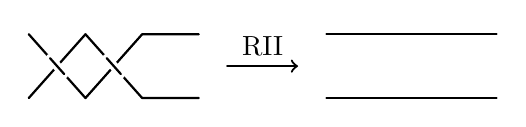
\begin{tikzpicture}[scale=0.9, line cap=round, line join=round]

% Reidemeister-II pair
\draw[line width=0.8pt]
    (0,0.45) -- (0.8,-0.45) -- (1.6,0.45) -- (2.4,0.45);
\draw[line width=0.8pt]
    (0,-0.45) -- (0.8,0.45) -- (1.6,-0.45) -- (2.4,-0.45);

% First crossing: upper strand
\draw[white,line width=3.2pt] (0.30,0.1125) -- (0.50,-0.1125);
\draw[line width=0.8pt]       (0.30,0.1125) -- (0.50,-0.1125);

% Second crossing: opposite strand is upper
\draw[white,line width=3.2pt] (1.10,0.1125) -- (1.30,-0.1125);
\draw[line width=0.8pt]       (1.10,0.1125) -- (1.30,-0.1125);

% Arrow
\draw[->,line width=0.8pt] (2.8,0) -- (3.8,0)
    node[midway,above] {$\mathrm{RII}$};

% After cancellation
\draw[line width=0.8pt] (4.2,0.45) -- (6.6,0.45);
\draw[line width=0.8pt] (4.2,-0.45) -- (6.6,-0.45);

\end{tikzpicture}

\small
Retained drawing with an incorrect second overpass: the illustrated arrow is not an allowed RII move. Valid RII removal requires the same physical strand to pass over at both crossings.
\end{center}

A valid RII cancellation preserves the raw regular-isotopy polynomial while removing two crossings. Reidemeister I changes the raw value by a monomial factor, and Reidemeister III does not reduce the crossing number. Removing an admissible pair changes the formal resolution space from $3^c$ to $3^{c-2}$.

The cancellation test searches for two crossings joined by the required pair of edges, verifies their adjacent incidence positions and compatible over/under parity, and follows the external arcs to determine the reconnection. The same physical strand must be over at both crossings. If the local pattern and reconnection are unambiguous, with the required distinct surviving endpoints, the two crossings and internal arcs are removed and the external arcs joined. Indices and smoothing connections are updated before another search. Adjacency alone is not sufficient, and the unchanged drawing is not evidence for the test's validity.

\paragraph{Organization of exact state merging}
The calculation can be described independently of a family-specific formula. First, compile and validate the diagram's incidence and crossing-resolution choices, and apply only admissible local reductions. Next, associate each surviving connectivity state with an exact Laurent-polynomial weight. Process the next crossing using the three terms of \Eqref{suppeq:yamada_local_relation}; update the corresponding connectivity and multiply the weight by $Y$, $Y^{-1}$ or $1$. Remove irrelevant label differences through the backend's canonical connectivity encoding, and combine only states with the same encoding by adding their exact weights. Once crossings are exhausted, evaluate the remaining crossing-free graph states with the graph-polynomial backend and sum their weighted contributions. Normalize the final polynomial only after the raw calculation, using the separate zero convention.

This specifies the mathematical organization of the optimization described here. The concrete compact-state encoding, canonicalization, traversal order and terminal graph evaluator are implementation choices available in the pinned source, rather than a new family-specific closed form. Time and memory depend on the number and size of distinct surviving states and polynomial coefficients, not on crossing count alone. A resource limit leaves an unavailable evaluation; it is not a valid zero and does not authorize abstract-polynomial substitution for an embedding-sensitive calculation.

\subsection{From exact evaluation to graph-family discovery}
\label{supp:yamada_discovery_bridge}
Published Yamada families illustrate the forward approach in which local structure is analyzed to obtain a recurrence or closed form. A generic evaluator permits a complementary data-driven approach: define a graph family, compute exact values, propose a relation and compare the relation with directly evaluated examples. In the subcubic families studied here, the intended workflow is
\begin{equation}
\boxed{\begin{aligned}
\text{define a spatial-graph family}&\longrightarrow\text{generate exact }\overline{\Upsilon}(G;Y)\text{ data}\\
&\longrightarrow\text{infer candidate relations}\longrightarrow\text{test additional family members}.
\end{aligned}}
\label{suppeq:yamada_discovery_bridge}
\end{equation}
A family formula is not required before obtaining the data. Conversely, a fit to those data does not establish the formula for every family member. The examples in \Figref{fig:three_theta_yamada_families} proceed from repeated motifs to commuting mixed words and ordered pure-braid words. The retrospective checks and the additional hypotheses required for all-family claims are developed in \SuppNoteref{supp:transfer_derivation}.
\FloatBarrier

\section{Validation across reconstruction, projection and invariant evaluation}
\label{supp:validation}
Reconstruction is tested against finite-thickness inputs generated from known graphs, projection through multi-view consistency and planar references, and the algebraic evaluator against graph identities and published formulas. These are separate tests of separate mathematical objects. Agreement at one stage does not certify the preceding correspondences.

\subsection{Algebraic and projection checks}
\label{supp:sanity_validation}
\begin{figure}[!t]
\centering
\includegraphics[width=\linewidth,keepaspectratio]{GeneralVersion/Figures/HandleBody_YamadaFramework_Stresstest.pdf}
\caption{\textbf{Representative reconstructions from graph-generated finite-thickness inputs.}
\textbf{(a--t)} Twenty retained examples from the recovery chain in \Eqref{suppeq:ground_truth_recovery}, with their historical graph-polynomial annotations. The stated benchmark construction uses a $200^3$ grid, tube radii of at least four voxels and thickness/safety factors of $0.90$. Its crossing-rich component was designed to comprise approximately $60\%$ of the ensemble, with at least two prescribed projected crossings and separation exceeding $2.4$ tube radii at those crossings. The input acceptance condition in \Eqref{suppeq:handlebody_betti} is a Betti-number consistency check, not a proof that every input is a handlebody. These selected panels do not establish a $100\%$ success rate for the full nominal $5{,}000$-construction ensemble; batch provenance and incomplete comparisons are discussed below.}
\label{suppfig:handlebody_stress}
\end{figure}

The tests separate four kinds of reference calculation.
\begin{enumerate}[leftmargin=*,label=\textbf{(\arabic*)}]
\item \textbf{Graph-level algebra.} Tested trees $T_1,\ldots,T_6$, cycles $C_1,\ldots,C_7$, bouquets $B_1,\ldots,B_6$ and theta graphs $\Theta_1,\ldots,\Theta_8$ are checked with the isthmus, one-point-union and edge-replacement identities \cite{kg_yamada1989,kg_li2018yamada}. Planar $K_4$ and further cubic values are compared with Dobrynin and Vesnin \cite{kg_dobrynin1996yamada}. The Negami backend is independently compared with the defining edge-subset polynomial \cite{kg_negami1987}, and its Yamada specialization with the direct graph evaluator.

\item \textbf{Published closed-form families.} For the $\Theta(n)$ family in \Figpanelref{fig:knottedgraph_topoly_scaling}{a,d,g}, Theorem~2 of Ref.~\cite{kg_dobrynin1996yamada} gives
\begin{equation}
\begin{aligned}
\Upsilon(\Theta(n);Y)={}&\left(Y^2+Y+1+Y^{-1}+Y^{-2}\right)Y^n
-\left(Y+Y^{-1}\right)Y^{-2n}
-\left(Y^2+1+Y^{-2}\right)(-1)^nY^{-n}.
\end{aligned}
\label{suppeq:dv_theta_oracle}
\end{equation}
For the edge-replaced families in \Figpanelref{fig:knottedgraph_topoly_scaling}{b,e,h}, let $\sigma(Y)=Y+1+Y^{-1}$. Theorem~5.1, Corollary~5.2 and Example~5.4 of Ref.~\cite{kg_li2018yamada} give
\begin{equation}
\Upsilon\!\left(C_n(\infty_+);Y\right)=\left[-Y^{-2}\sigma(Y)\right]^n+\sigma(Y)\left(Y^{-2}+1\right)^n,
\label{suppeq:li_cycle_oracle}
\end{equation}
and for the corresponding theta construction,
\begin{equation}
\Upsilon\!\left(\Theta_s(\infty_+);Y\right)=\frac{[-\sigma(Y)]^s+\sigma(Y)\left[(\sigma(Y)+1)Y^{-2}+1\right]^s}{1+\sigma(Y)}.
\label{suppeq:li_theta_oracle}
\end{equation}
The stored tested examples agree with these references, including structured diagrams with $500$ crossings. This is a demonstrated input scale for the particular families, not a claim that all diagrams of that size have comparable cost. Topoly~1.1.0 \cite{kg_topoly2021} is compared only where both programs satisfy the same reference polynomial. The representative $25\times$, $136\times$ and $567\times$ ratios refer to these matched reference-passing cases, not to absent or skipped comparator results.

\item \textbf{Crossings and mirroring.} Planar theta, crossed-theta and mirror examples test crossing-sensitive behavior. The one-crossing factor $(-Y)^{\pm1}$ is compared with the convention used in Ref.~\cite{kg_peddada2023}.

\item \textbf{Projection consistency.} Each accepted view of a fixed subcubic embedding is independently processed through crossing detection, height assignment and PD construction. Normalized outputs must agree even if the diagrams have different crossing counts. Planar references also admit a crossing-free calculation. The tested catalogue includes theta, $K_4$, triangular-prism, $K_{3,3}$ and cube-type examples. Equal outputs are consistency checks, not a complete equivalence decision for arbitrary independently supplied graphs.
\end{enumerate}

\paragraph{Available scaling-benchmark protocol}
The retained benchmark implementation makes one timed invariant call per requested graph/framework pair in a fresh spawned worker. It has no explicit warmup or repeated-measurement distribution. The worker clock starts immediately before framework evaluation and stops after conversion to the comparison coefficient dictionary. Geometry construction, projection, worker startup and result serialization lie outside this worker timer. The recorded \texttt{KnottedGraph} route uses the raw invariant with \texttt{normalize=False}, \texttt{n\_jobs=1} and \texttt{method="negami"}. The comparator clears its process-global Yamada memo table inside its timed function. Projection preprocessing can be reused from a geometry/PD cache, and retained Topoly ledger results can be reused rather than freshly timed.

The currently documented requested limits are $600\,\mathrm{s}$ for \texttt{KnottedGraph} and $100{,}000\,\mathrm{s}$ for Topoly; these controls do not establish that every missing historical point consumed that budget. Some later family points are explicitly skipped after a comparator non-pass. The 112-row comparison ledger does not supply a historical CPU/RAM specification, operating system, complete dependency versions, compiler flags, measured thread-environment values or per-row source commit. These missing fields are not filled with the machine information of a later audit. The quoted historical timings are therefore limited to their retained protocol and samples; no repeated-run error bar, memory bound or hardware-independent scaling conclusion is inferred. The relevant audit and script identifiers are listed in \SuppSubsecref{supp:reproducibility_resources}.

\subsection{Handlebody--spatial-graph reconstruction tests}
\label{supp:handlebody_validation}
The inverse test begins with a known embedded graph and a geometrically generated thickening:
\begin{equation}
G_i\longrightarrow\Omega_i=N(G_i)\longrightarrow\Omega_i^{\mathrm{voxel}}\longrightarrow G_i^{\mathrm{rec}}.
\label{suppeq:ground_truth_recovery}
\end{equation}
Connected components and lattice Euler characteristics are computed using SciPy and \texttt{scikit-image} \cite{kg_virtanen2020scipy,kg_vanderwalt2014skimage}, with the chosen digital Euler convention \cite{kg_ohser2002euler}. \SuppFigref{suppfig:handlebody_stress} retains twenty illustrative outputs. Their presentation does not identify a complete, uniformly successful $5{,}000$-row invariant ledger.

\begin{center}
\fbox{\begin{minipage}{0.92\linewidth}
\textbf{Inverse reconstruction protocol and distinct checks}
\begin{enumerate}[leftmargin=*,label=\textbf{\arabic*.},itemsep=3pt,topsep=4pt]
\item \textbf{Generate a graph.} Construct a connected bridge-free subcubic embedded graph $G_i$. For the crossing-rich generators, check the prescribed crossings in the standard $xy$ view and require centerline separation $d_{\min}>2.4\,r_{\mathrm{tube}}$ at those crossings.
\item \textbf{Thicken and voxelize.} Estimate non-contact separation by dense edge resampling, excluding shared-junction neighborhoods for incident edges, and choose a tube radius $r_i$. The intended geometric neighborhood is
\begin{equation*}
\Omega_i=N_{r_i}(G_i)=\{\mathbf x\in\mathbb R^3:\operatorname{dist}(\mathbf x,G_i)\leq r_i\}.
\end{equation*}
Place a $200^3$ grid around the embedding with an additional margin $2.25r_i$. For a segment $[\mathbf a,\mathbf b]$, the nearest point to a voxel center is
\begin{equation*}
\mathbf c=\mathbf a+\operatorname{clip}_{[0,1]}\!\left[\frac{(\mathbf x-\mathbf a)\cdot(\mathbf b-\mathbf a)}{\|\mathbf b-\mathbf a\|^2}\right](\mathbf b-\mathbf a).
\end{equation*}
The voxel is occupied if $\|\mathbf x-\mathbf c\|\leq r_i$ for at least one segment. A sampled clearance estimate is not an exact regular-neighborhood certificate.
\item \textbf{Check digital topology and thickness.} Accept the benchmark input when
\begin{equation}
\bigl(\beta_0(\Omega_i^{\mathrm{voxel}}),\beta_1(\Omega_i^{\mathrm{voxel}}),\beta_2(\Omega_i^{\mathrm{voxel}})\bigr)=\bigl(1,\beta_1(G_i),0\bigr)
\label{suppeq:handlebody_betti}
\end{equation}
and the tube radius is at least four voxels. This is a necessary consistency check for the intended topology. It does not prove manifoldness, handlebody structure or ambient-isotopic source correspondence.
\item \textbf{Reconstruct.} Apply the stated extraction and cleanup sequence to obtain $G_i^{\mathrm{rec}}$, retaining its incidence and polylines.
\item \textbf{Check graph summaries.} Record connectedness, subcubic valence and $\beta_1(G_i^{\mathrm{rec}})=\beta_1(G_i)$. Record abstract multigraph isomorphism separately rather than conflating it with equal cycle rank.
\item \textbf{Compare embedding-sensitive values.} When both computations complete in the admissible convention, compare
\begin{equation*}
\overline{\Upsilon}_{\mathrm{seed}}=\overline{\Upsilon}(G_i;Y),\qquad
\overline{\Upsilon}_{\mathrm{rec}}=\overline{\Upsilon}(G_i^{\mathrm{rec}};Y).
\end{equation*}
Equality is an invariant-consistency result, not a sufficient proof of ambient isotopy. Missing computations are not matches, and a mismatch is retained.
\item \textbf{Report outcomes separately.} Distinguish attempted inputs, accepted digital masks, graph-summary passes, polynomial attempts, completed comparisons, matches, mismatches and unverified records. An overall Boolean flag must not replace these counts.
\end{enumerate}
\end{minipage}}
\end{center}

\paragraph{Historical batch evidence and its limits}
The available neighboring preservation CSV inspected in the 18 September audit has $5{,}000$ passing input-summary checks and $5{,}000$ passing primary graph-summary checks. Its invariant column contains $4{,}472$ matches, one mismatch and $527$ blank comparisons; the overall flag has $4{,}999$ passes and one failure. Abstract isomorphism is true in $680$ rows and false in $4{,}320$. The mismatch is associated with \texttt{random\_4920}: the seed and reconstruction have different vertex/edge counts but equal cycle rank. These outcomes demonstrate why the graph-summary condition cannot stand in for invariant or embedding recovery.

The inspected CSV was not conclusively matched to the manuscript's historical timing artwork. Its counts are therefore reported as the audited available batch, not substituted as a newly established success rate for every retained figure panel. Blank comparisons are unverified, not assumed failures or matches. Later replay records can only be associated with the historical ensemble after input identities and source metadata are matched; such a replay is not automatically a fresh reconstruction. This version withdraws the earlier statement that every case recovered its spatial topology whenever evaluated. Individual benchmark manifests, completed checks and unresolved associations must be read with their own provenance.

\begin{figure*}[!t]
\centering

\includegraphics[width=\linewidth,keepaspectratio]{./GeneralVersion/Figures/Time_distributions.pdf}
\caption{\textbf{Retained historical per-stage timing distributions.}
\textbf{(a)} Voxel skeletonization; \textbf{(b)} graph extraction; \textbf{(c)} short-edge contraction; \textbf{(d)} leaf removal; \textbf{(e)} degree-two simplification; \textbf{(f)} Ramer--Douglas--Peucker smoothing; \textbf{(g)} projection selection; \textbf{(h)} \texttt{KnottedGraph} invariant evaluation; and \textbf{(i)} completed external Topoly evaluations. Solid and dashed lines display the original means and 95th percentiles. The figure is retained unchanged as descriptive historical output. A common matched sample set and complete original-run provenance for all panels have not been established; in particular, the invariant panels must not be interpreted as a paired speedup estimate. The annotations are not fresh measurements of the corrected release or a $5{,}000$-case invariant-success certificate.}
\label{suppfig:handlebody_timing_distributions}
\end{figure*}

The histograms in \SuppFigref{suppfig:handlebody_timing_distributions} visualize the different operations in \SuppFigref{suppfig:skeletonization_steps}. Their retained annotations include means near $0.052\,\mathrm{s}$ for skeletonization, $0.031\,\mathrm{s}$ for projection selection, $0.024\,\mathrm{s}$ for contraction, $0.013\,\mathrm{s}$ for simplification and smoothing, and $6.6\times10^{-5}\,\mathrm{s}$ for leaf removal. These are descriptions of the unchanged plotted summaries, not independently reproduced estimates with newly established cohorts.

The two invariant panels show means near $1.1\times10^{-3}\,\mathrm{s}$ and $3.63\,\mathrm{s}$ among their respective recorded outcomes. Their ratio is not used as a measured paired acceleration: completion policies and cohort correspondence must first be matched, and failed, skipped and resource-limited calls must be separated. The reference-gated structured-family comparisons in \Figref{fig:knottedgraph_topoly_scaling} supply the narrower performance evidence used in the main text. Missing historical hardware, per-panel sample membership, timing boundaries and timeout metadata remain explicit limitations rather than being inferred from the visual separation of these distributions.
\FloatBarrier

\section{Exploratory parameter scans of finite-thickness geometries}
\label{supp:knot_fields}
The shared interfaces can be applied repeatedly to a family of regions $\Omega_{\boldsymbol\theta}$:
\begin{equation}
\boldsymbol\theta\longmapsto\Omega_{\boldsymbol\theta}\longmapsto G_{\boldsymbol\theta}\longmapsto\mathcal S(G_{\boldsymbol\theta}).
\label{suppeq:generic_phase_map}
\end{equation}
Here $G_{\boldsymbol\theta}$ is a numerical graph representation and $\mathcal S$ is the explicitly stated graph, diagram or audit signature. Equal signatures do not establish equivalence of the continuous regions, and changes between neighboring signatures are not automatically topology-changing boundaries of the source. This distinction applies even before display filtering, because extraction can change the represented graph and a selected spine's ordinary Yamada polynomial is not invariant under every admissible change of spine.

The figures in this note are retained from the historical exploratory scans without changing their artwork. Their plotted labels include postprocessing and are not presented as corrected, unfiltered invariant maps. The source definitions and filtering rules below explain what the retained images display and which previous interpretations are withdrawn. Later audit calculations referenced in \SuppSubsecref{supp:reproducibility_resources} are separate records; they are not silently substituted as the numerical source of these images.

\begin{figure}[!t]
\centering

\includegraphics[width=\linewidth]{GeneralVersion/Figures/PhaseDIagrams.pdf}
\caption{\textbf{Historical, postprocessed Hamiltonian scan displays.}
The five panels correspond to \textbf{(a)} Hopf link $\rightarrow$ trefoil, \textbf{(b)} Hopf link $\rightarrow$ Solomon link, \textbf{(c)} unknot $\rightarrow$ trefoil, \textbf{(d)} unknot $\rightarrow$ Solomon link and \textbf{(e)} trefoil $\rightarrow$ cinquefoil. The original grid contains $7{,}140$ parameter points. Its $60$ inclusive interpolation samples have spacing $1/59$, and the retained energy array has spacing $99/980\simeq0.1010204$, not exactly $0.1$. The unchanged color bar labeled $\Upsilon$ and the black boundaries encode the legacy grouping and display procedure, which mixed evaluation scopes and relabeled small regions. They must not be read as uniformly normalized spatial Yamada values, a certified source-solid phase classification or located Lifshitz transitions. The finite-domain and historical postprocessing conventions are stated in \SuppSubsecref{supp:hamiltonian_phase_maps}.}
\label{suppfig:additional_phase_diagrams}
\end{figure}

\subsection{Hamiltonian-derived finite-thickness momentum-space regions}
\label{supp:hamiltonian_phase_maps}
Finite-energy Fermi volumes motivate parameter-dependent geometric analysis. Lifshitz transitions concern changes in Fermi-surface topology \cite{kg_lifshitz1960,kg_varlamov2021lifshitz}; strain and pressure can tune such transitions \cite{kg_sunko2019lifshitz,kg_xiang2015lifshitz}. Composition is another way to tune a Hamiltonian and its band topology \cite{kg_dziawa2012topological}, but a composition-driven topological crystalline transition is not identified with a Fermi-surface Lifshitz transition merely by that citation. The companion work addresses a Fermi-volume spatial-graph construction \cite{akgun_yan_2026topologicalclassificationknottedgraphs}. The retained scans here illustrate use of the software on analytic benchmark inputs, not an independent validation of all continuum phase boundaries.

The constructor family uses
\begin{equation}
\begin{aligned}
z(\mathbf k)&=\cos(2k_z)+c_0+i\!\left(\cos k_x+\cos k_y+\cos k_z-m\right),\\
w(\mathbf k)&=\sin k_x+i\sin k_y,\\
f_{p,q}(\mathbf k)&=z(\mathbf k)^p-w(\mathbf k)^q,
\end{aligned}
\label{suppeq:nodal_pq_field}
\end{equation}
with the Hermitian reference Hamiltonian
\begin{equation}
H_{p,q}(\mathbf k)=\operatorname{Re}f_{p,q}(\mathbf k)\,\sigma_x+\operatorname{Im}f_{p,q}(\mathbf k)\,\sigma_z.
\label{suppeq:nodal_pq_hamiltonian}
\end{equation}
The complex nodal construction follows Refs.~\cite{kg_bi2017nodalknot,kg_lee2020nodalknots}. The constructor labels unknot, Hopf link, trefoil, Solomon link and cinquefoil refer to $(p,q)=(1,1),(2,2),(2,3),(2,4),(2,5)$. These names do not by themselves certify every sampled finite-window nodal embedding.

The recovered implementation uses $m=2$. Most endpoints use $c_0=0.5$, whereas the Solomon endpoint uses the numerical constant $c_0=0.333$, not the exact rational $1/3$. Thus interpolation to Solomon combines endpoint Hamiltonians with different coordinate-map constants. The parameter $c_0$ is distinct from the TPMS threshold $c$ below.

The Hermitian positive band is $\varepsilon_{p,q}(\mathbf k)=|f_{p,q}(\mathbf k)|$. With all sets in this subsection restricted to the finite sampled domain specified below, write
\begin{equation}
\Omega_{\lambda,E}=\{\mathbf k:\varepsilon_\lambda(\mathbf k)\leq E\},
\label{suppeq:fermi_volume_phase_map}
\end{equation}
where $\varepsilon_\lambda$ is the positive band of
\begin{equation}
H_\lambda(\mathbf k)=(1-\lambda)H_0(\mathbf k)+\lambda H_1(\mathbf k),\qquad 0\leq\lambda\leq1.
\label{suppeq:phase_map_interpolation}
\end{equation}
The numerical route actually uses an auxiliary non-Hermitian model with an additional $i\Gamma\sigma_y$ term. For real coefficients $d_1,d_3$ of the other Pauli matrices and $\Gamma>0$, its exceptional-volume condition corresponds in exact arithmetic to $d_1^2+d_3^2\leq\Gamma^2$. This is the same geometric sublevel condition as the Hermitian positive-band region at $E=\Gamma$. The equivalence concerns the selected geometry, not a claim that the computational Hamiltonian itself is Hermitian. The historical mask implements a zero-real-spectrum condition; numerical extraction and boundary treatment still require separate checks.

The sampled box is $W=[-\pi,\pi]\times[-\pi,\pi]\times[0,\pi]$, at $120^3$ resolution, with displayed coordinate scaling $(1,1,2)$. No periodic face-identification operation was established for this route. In particular, the simultaneous appearance of $\cos k_z$ and $\cos 2k_z$ does not make $[0,\pi]$ a periodic fundamental interval for the complete field. Boundary-touching masks are finite-window objects, not silently closed by identifying opposite faces.

The recovered candidate arrays are
\begin{equation}
\lambda_j=\frac{j}{59},\quad j=0,\ldots,59,
\qquad E_k=0.30+\frac{99}{980}k,\quad k=0,\ldots,49.
\label{suppeq:hamiltonian_sampling}
\end{equation}
Panels \textbf{(a,c)} retain $16$ energy values, \textbf{(b,d)} retain $24$, and \textbf{(e)} retains $39$. The largest retained energies are approximately $1.8153061$, $2.6234694$ and $4.1387755$, respectively, and the total is $60(16+24+16+24+39)=7140$. The historical terminal-row rule stopped or cropped at the first energy row classified as a one-vertex result for every interpolation sample. This was an algorithmic criterion, not a demonstrated physical transition.

\paragraph{Historical grouping and display postprocessing}
The retained scan route mixed spatial and abstract graph-polynomial calculations through a fallback that could replace a failed projected evaluation with an abstract result. Its original per-cell outputs do not establish which calls used that fallback. Consequently, the unchanged figure is not assigned the uniform interpretation $\mathcal S=\overline{\Upsilon}$ in the ambient-isotopy sense.

The historical parameter-space filter additionally selected four-connected components smaller than $\max(5,\lceil0.01N_{\mathrm{panel}}\rceil)$ and iteratively reassigned them to neighboring large-component labels. Votes used eight neighboring pixels, with total label area and then label index as tie breakers. Small area alone does not demonstrate numerical noise. Abstract-contraction grouping and the filter can both merge labels without establishing equality of spatial embeddings. Neither a black boundary in the retained image nor a constant-color region is therefore used as a certified continuum transition or topology-preserving corridor.

For an independently validated source family, actual Fermi-surface topology changes can affect density of states \cite{kg_galeski2022lifshitz,kg_ichinokura2022lifshitz}, transport \cite{kg_galeski2022lifshitz}, thermodynamics \cite{kg_slizovskiy2015lifshitz} and superconducting behavior \cite{kg_shi2017lifshitz}. These references motivate the application; they do not identify the boundaries of the historical figure as such transitions. Extension to multiband material Hamiltonians similarly requires an explicit band or gap condition, boundary convention and validated source-to-graph correspondence. No result for a particular material is inferred solely from this exploratory benchmark display.

\subsection{TPMS-derived solids: graph grouping and reconstruction limits}
\label{supp:tpms_phase_maps}
\label{sec:tpms_design_maps}

\begin{figure*}[t!]
\centering

\includegraphics[width=0.88\linewidth]{GeneralVersion/Figures/PorousMaterialPhaseMap.pdf}
\caption{\textbf{Historical filtered grouping of numerically reconstructed TPMS-derived graphs.}
\textbf{(a)} Schwarz-P $\rightarrow$ Diamond, \textbf{(b)} Gyroid $\rightarrow$ Schwarz-P and \textbf{(c)} Gyroid $\rightarrow$ Diamond. Colors follow a bounded abstract-contraction grouping and a subsequent small-region display filter, not a demonstrated equivalence of spatial embeddings. The filter changes $18$, $67$ and $86$ distinct cells, respectively ($171$ of $1{,}323$). The stored scan also mixes polynomial and graph/audit outputs, with normalization and valence limitations detailed in the text. Black boundaries separate final display labels rather than certified source-topology phases. \textbf{(d)} The five retained geometries and interval labels at $c=0.105$ illustrate that filtered display; they are not five proved topological regimes. Transparent surfaces, black graph curves and red vertices are unchanged historical renderings. This figure is retained for illustration of the numerical workflow, not as evidence for the withdrawn $3/11/14$ topological-class interpretation.}
\label{fig:tpms_phase_maps}
\end{figure*}

TPMS-derived geometries are used as templates for lightweight structures \cite{kg_maskery2018tpms}, tissue scaffolds \cite{kg_castro2019tpms_permeability,kg_liu2022tpms_topological_design} and thermal-management devices \cite{kg_gado2024tpms}. Architecture can influence permeability and mechanical response at comparable occupied fraction. These studies motivate examining network structure as well as density; they do not validate the grouping or filtered boundaries in the present retained illustration.

The numerical scan has the form
\begin{equation}
(\lambda,c)\longmapsto\Omega_{\lambda,c}\longmapsto G_{\lambda,c}\longmapsto\mathcal S(G_{\lambda,c}),
\label{suppeq:tpms_phase_map}
\end{equation}
where $\mathcal S$ denotes the historical operational record, not a complete spatial-graph or handlebody invariant. A graph-only reduction is appropriate only when its required source correspondence is established. It is not inferred from surface closure or the absence of contact with the outer computational box.

The three fields are
\begin{equation}
\begin{aligned}
F_{\mathrm G}(x,y,z)&=\sin x\cos y+\sin y\cos z+\sin z\cos x,\\
F_{\mathrm P}(x,y,z)&=\cos x+\cos y+\cos z,\\
F_{\mathrm D}(x,y,z)&=\cos x\cos y\cos z-\sin x\sin y\sin z.
\end{aligned}
\label{suppeq:tpms_fields}
\end{equation}
They are nodal approximations used in Gyroid, Schwarz-P and Diamond design \cite{kg_gado2024tpms}, not a claim that every blend or nonzero level is an exact minimal surface. For selected endpoints,
\begin{equation}
F_\lambda=(1-\lambda)F_A+\lambda F_B,\qquad0\leq\lambda\leq1.
\label{suppeq:tpms_interpolation}
\end{equation}
The isosurface $F_\lambda=c$ and sublevel set $F_\lambda\leq c$ define the geometric template and the selected occupied region. Related combinations of canonical fields occur in hybrid-architecture design \cite{kg_mele2025hybrid_tpms}. The interpolation parameter and threshold describe geometric control variables, not predefined topological class labels.

The periodic fields are restricted to a finite spherical domain. The implementation uses $R=0.72(2.25\pi)\simeq5.08938$ within $[-2.25\pi,2.25\pi]^3$, with its numerical value stored at machine precision. The finite solid is
\begin{equation}
\Omega_{\lambda,c}=\{\mathbf r:F_\lambda(\mathbf r)\leq c,\ \|\mathbf r\|\leq R\}.
\label{suppeq:tpms_compact_solid}
\end{equation}
It can also be described by
\begin{equation}
\Psi_{\lambda,c}(\mathbf r)=\max\!\left[F_\lambda(\mathbf r)-c,\frac{\|\mathbf r\|}{R}-1\right],
\qquad\Omega_{\lambda,c}=\{\mathbf r:\Psi_{\lambda,c}(\mathbf r)\leq0\}.
\end{equation}
The max expression records the intersection; it is not a globally smooth function to which an unconstrained Morse argument can be applied at the joining boundary. Interior and spherical-wall events must instead be treated separately.

The historical figure uses the three paths $F_{\mathrm P}\to F_{\mathrm D}$, $F_{\mathrm G}\to F_{\mathrm P}$ and $F_{\mathrm G}\to F_{\mathrm D}$, with $21$ inclusive values each of $\lambda\in[0,1]$ and $c\in[0,0.3]$. The spacings are $0.05$ and $0.015$. At $64^3$ spatial resolution this gives $1323$ sampled compact volumes. The recorded surfaces are closed and do not touch the computational-box boundary, but the spherical cutoff is itself part of the object's boundary and can contribute constrained events.

\paragraph{What the retained color map actually groups}
The comparison converted stored geometry to \texttt{networkx.MultiGraph} incidence data and tested abstract isomorphism after non-loop contractions. Spatial coordinates were not part of that comparison. The bounded search used up to $1000$ states, depth three and a 24-edge limit per test. Its labels are thus operational groups of extracted abstract graphs; they do not establish equivalence of knotted embeddings or their regular neighborhoods. A failed bounded comparison establishes only that the search did not find the requested relation within those limits. The spatial-contraction theorem in \SuppSubsecref{supp:handlebody_basis} does not justify replacing its spatial moves by this abstract procedure.

The stored $1323$ records contain $614$ entries labeled \texttt{yamada}, $636$ labeled \texttt{large-core} and $73$ labeled \texttt{vertex}. These source labels are bookkeeping rather than interchangeable invariants. In the audited historical batch, all $614$ polynomials have nonzero minimum degree: $513$ have degree $-5$ and $101$ degree $-7$. They are therefore not normalized as in \Eqref{suppeq:yamada_normalization}. Of the polynomial-labeled records, $37$ involve degree-greater-than-three vertices, so their interpretation also requires retaining the diagram/vertex structure. In $17$ records, the stated volume and graph component counts differ. Such a discrepancy is incompatible with a retraction of the entire volume under common conventions and cannot be ignored when calling the output a spine.

The referenced historical evaluator could silently return an abstract graph polynomial after a spatial-evaluation exception. The retained records do not identify every call that used that path, and no retrospective fallback count is invented. Nor is the fallback assumed to explain the normalization or component discrepancies without a corresponding trace. Consequently, zero recorded outer errors is not evidence that all spatial computations succeeded. The unchanged map is not used as quantitative evidence of normalized spatial classes.

\paragraph{Display filtering and the withdrawn class interpretation}
After abstract grouping, a further filter replaced connected regions with fewer than four parameter cells by the most frequent neighboring label, for up to three passes. This additional, order-dependent spatial relabeling is not described adequately by ``contraction stabilization.'' The audited changes are
\begin{table}[!t]
\centering\small
\begin{tabular}{lrrr}
\hline
Path & Before filter: labels/regions & Displayed: labels/regions & Changed cells\\\hline
Schwarz-P $\to$ Diamond & $15/19$ & $3/3$ & $18$\\
Gyroid $\to$ Schwarz-P & $20/64$ & $11/16$ & $67$\\
Gyroid $\to$ Diamond & $52/88$ & $14/15$ & $86$\\\hline
\end{tabular}
\caption{\textbf{Documented postprocessing of the unchanged TPMS display.} Counts refer to operational labels and connected parameter-grid regions, not established topological classes. The last column counts distinct cells whose final label differs, totaling $171$; the corresponding $18$, $71$ and $94$ reassignment operations can revisit a cell.}
\label{supptab:tpms_filter}
\end{table}

The displayed $3/11/14$ label counts, $3/16/15$ region counts and the five interval annotations in \SuppFigpanelref{fig:tpms_phase_maps}{d} are therefore not claimed as topology conclusions. The figure is preserved as a historical filtered illustration. Small filtered regions have not been demonstrated to be noise, and a constant display label is not a certified optimization corridor. Corrected software records, unfiltered audits and changed-cell information in the cited repository are separate evidence rather than a retroactive change to these retained pixels.

\paragraph{Independent critical-point analysis: a separate validation target}
For a smooth scalar sublevel set on a compact domain, the absence of level-critical points and appropriate boundary tangencies supplies regularity conditions for continuation \cite{kg_milnor1963morse}. At fixed $\lambda$, candidate interior events obey
\begin{equation}
\nabla F_\lambda(\mathbf r_*)=0,\qquad c_*(\lambda)=F_\lambda(\mathbf r_*).
\label{suppeq:tpms_morse_discriminant}
\end{equation}
The spherical wall adds constrained candidates,
\begin{equation}
\nabla F_\lambda(\mathbf r_*)=\eta\mathbf r_*,\qquad\|\mathbf r_*\|=R,\qquad c_*=F_\lambda(\mathbf r_*).
\label{suppeq:tpms_boundary_critical}
\end{equation}
These equations specify an independent source-geometric problem. Their critical-value branches are not identified with the black boundaries of the filtered image. A stationary event can be degenerate, several events can share a critical value, and a Hessian index gives the local attachment type rather than a complete global classification without attachment information. Later certified-continuation work in the research records is an independent audit and is not what the unchanged figure plots.

A local neck model remains useful as a prospective interpretation after an actual nondegenerate event has been established. For an index-one point, with $\kappa_i>0$,
\begin{equation}
F_\lambda-c_*\simeq\frac12\left(-\kappa_1u^2+\kappa_2v^2+\kappa_3w^2\right).
\label{suppeq:tpms_local_index_one}
\end{equation}
At $u=0$, $\delta=c-c_*>0$ gives $\kappa_2v^2+\kappa_3w^2\leq2\delta$ and hence
\begin{equation}
A_{\mathrm{neck}}\simeq\frac{2\pi\delta}{\sqrt{\kappa_2\kappa_3}},\qquad r_{\mathrm{neck}}\propto\sqrt\delta.
\label{suppeq:tpms_neck_scaling}
\end{equation}
This is a local geometric consequence of the assumed normal form, not a measured property of every displayed boundary. Under a further fixed-effective-length, Poiseuille-like cylindrical-throat model, hydraulic conductance would scale as $r^4\sim\delta^2$. A slender solid bridge with fixed characteristic length would instead have axial stiffness or solid thermal conductance proportional to area, and bending rigidity proportional to a fourth moment. Those additional model assumptions need not describe an actual evolving TPMS neck; no macroscopic transport or mechanical exponent is inferred here.

Replacing $F_\lambda$ by $-F_\lambda$ reverses Hessian signs, interchanging local Morse indices $k$ and $3-k$. This relates local solid and complementary-phase descriptions, but does not by itself predict whether a global network gains a component, handle or transport pathway. Mechanical, permeability and thermal studies \cite{kg_maskery2018tpms,kg_castro2019tpms_permeability,kg_santos2020tpms_permeability,kg_liu2022tpms_topological_design,kg_gado2024tpms} motivate future response calculations for independently validated geometries; they do not establish response changes for these historical map labels.

A prospective robustness margin could be defined as
\begin{equation}
\rho_{\mathrm{top}}(\lambda,c)=\operatorname{dist}_{\mathrm{norm}}\!\left[(\lambda,c),\partial\mathcal P_{\mathrm{top}}\right],
\label{suppeq:tpms_topological_margin}
\end{equation}
where $\partial\mathcal P_{\mathrm{top}}$ would have to be an independently justified transition set and the parameter metric explicitly specified. That set has not been determined by the retained filtered image, so no numerical manufacturing tolerance, topology-preserving design corridor or inverse-design guarantee is obtained from it. Spatially graded controls introduce additional interfaces and cannot be certified solely by assigning each local parameter value a color from a homogeneous scan.

The same interfaces could be explored for other finite-thickness inputs, including ion-density level sets around topological colloids \cite{kg_everts2018doublelayer}, toroidal-droplet simulations \cite{kg_wu2024torusdroplets}, nematic-droplet transitions \cite{kg_koizumi2023nematic} and cavitation geometries \cite{kg_wang2014bubble,kg_wang2015bubble}. These are prospective applications, not additional validations in this manuscript. Each requires its own source interpretation, boundary convention and reconstruction checks before a spatial-graph signature can be related to the continuous physical geometry.
\FloatBarrier

\section{Geometric preconditioning of difficult embeddings}
\label{supp:repulsive_layout}
An embedding can be difficult to project even when its incidence and intended topology are fixed. Noisy coordinates, clustered vertices, long detours and near contacts can create avoidable crossings or unresolved views. The optional preconditioning module changes coordinates while retaining graph identity and returns the result to the common embedded-graph interface (\Figpanelref{fig:functionality_overview}{f}). The nonlocal objective belongs to the tangent-point energy family, with an early formulation by Buck and Orloff \cite{kg_buck1995energy}, and follows the computational framework of Yu, Schumacher and Crane \cite{kg_yu2021repulsive}.

The native solver can use Henrik Schumacher's \texttt{Repulsor}. The third-party notice in the immutable software reference listed in Code availability specifies revision \texttt{adc56b61f65f5958b59cbd7e1539f44ed0c5e993}; the upstream source is \url{https://github.com/HenrikSchumacher/Repulsor}. This pin identifies the documented reproducibility dependency, not independently recovered execution metadata for every historical figure. Geometry-to-curve mappings, pinned junctions and optional swept-step checks connect the optimizer to the graph representation without treating repulsion alone as a topology certificate.

\subsection{Simplifying graphs with repulsive curves}
\label{supp:repulsive_objective}
The graph is converted to a curve network while retaining mappings from curve samples to graph vertices and edges. Vertices can be pinned, with optional collar points on incident edges. Resampling or optional guarded decimation controls the number of samples. The inverse mapping preserves node labels, edge keys and non-geometric attributes when the final curve is returned to a \texttt{MultiGraph}.

Let $\mathcal X=\{\mathbf x_i\}\subset\mathbb R^3$ be the curve samples, $\mathcal S$ its segments and $\mathcal P\subset\mathcal S\times\mathcal S$ the pairs included in the nonlocal sum. For $s=[\mathbf x_i,\mathbf x_j]$, denote its length by $\ell_s$, midpoint by $\mathbf c_s$, unit tangent by $\boldsymbol\tau_s$ and normal projector by $\Pi_s^\perp=I-\boldsymbol\tau_s\boldsymbol\tau_s^T$. The discrete energy is
\begin{equation}
E_{\mathrm{tp}}^{p,q}(\mathcal X)=\sum_{(s,t)\in\mathcal P}\ell_s\ell_t\frac{\|\Pi_s^\perp(\mathbf c_t-\mathbf c_s)\|^q+\|\Pi_t^\perp(\mathbf c_s-\mathbf c_t)\|^q}{\|\mathbf c_t-\mathbf c_s\|^p}.
\label{suppeq:tangent_point_energy}
\end{equation}
The displayed examples use $p=8$ and $q=4$. Optional local terms include
\begin{equation}
E_{\mathrm{len}}=\sum_{s\in\mathcal S}\ell_s^2
\end{equation}
and
\begin{equation}
E_{\mathrm{bend}}=\sum_i\|\mathbf x_{i-1}-2\mathbf x_i+\mathbf x_{i+1}\|^2,
\end{equation}
together with an optional clearance penalty for non-adjacent strands. Their weights are user-controlled; neither a common degree of compaction nor a particular geometric interpretation is imposed on every scientific input.

\subsection{Relaxation and topology checks}
\label{supp:repulsive_topology}
A repulsive objective is not by itself a guarantee of ambient isotopy. Proposed updates use a maximum-safe-step estimate, a user-controlled safety fraction and backtracking. The public graph route pins vertices by default unless they are explicitly released. When the intermediate motion states needed for independent verification are retained, the verifier can replay the trajectory and test swept segments. A failed verification is not reported as successful topology preservation.

Static clearance statistics for the initial, relaxed and decimated configurations are separate geometric diagnostics. They do not rule out strand intersections during the intervening motion. Likewise, a geometric shortcut requires its own check: the guarded decimation route tests the swept triangle against non-adjacent segments. Any claim of preservation applies to the operations actually checked, their numerical tolerances and the recorded trajectory; it is not inferred from an unchanged abstract graph. Solver parameters, step history, clearance statistics, scale, length and graph--curve mappings are retained when available.

\begin{figure}[!t]
\centering
\includegraphics[width=\linewidth]{GeneralVersion/Figures/Repulsive_curves.pdf}
\caption{\textbf{Optional geometric preconditioning before projection.}
Each row retains a protein-derived example from the RCSB Protein Data Bank \cite{kg_burley2019rcsb}, through unfolding, compaction, smoothing, projection and PD/polynomial evaluation. The tangent-point term in \Eqref{suppeq:tangent_point_energy} uses $p=8$, $q=4$ for these examples \cite{kg_yu2021repulsive}. The unchanged artwork illustrates coordinate processing and return to the common graph interface. Incidence retention, static strand separation and verified swept-motion preservation are distinct properties; the images alone do not certify an unarchived intermediate trajectory.}
\label{suppfig:repulsive_curves_pipeline}
\end{figure}

\subsection{Return to the common graph and projection pipeline}
\label{supp:repulsive_return}
In the displayed examples, nonlocal repulsion first opens close contacts, length control removes detours while repulsion remains active, and local terms regularize the final curves. This staging is a figure-generation choice rather than a required sequence in every public call. Updated node positions and polylines are mapped onto a copy of the original graph, retaining labels, edge keys and non-geometric attributes. Optional final simplification is a separate operation whose admissibility must be checked rather than assumed from the preceding relaxation. The returned graph uses the same projection and invariant interfaces as an unrelaxed input. Preconditioning is a numerical aid, not a replacement for independent diagram or invariant checks.
\FloatBarrier

\section{\texttt{KnottedGraph} supports evaluator-guided mathematical discovery}
\label{supp:transfer_derivation}
The exact evaluator also provides a data layer for investigating parameterized spatial-graph families. This problem has substantial prior mathematical structure. Dobrynin and Vesnin derive an all-$n$ formula for a family of knotted two-vertex cubic graphs \cite{kg_dobrynin1996yamada}. Li, Lei, Li and Vesnin derive edge-replacement formulas \cite{kg_li2018yamada}; associated work analyzes families whose polynomial roots are dense in the complex plane \cite{kg_li2019density}. Lundstr\"om develops transfer-matrix calculations for repeated symmetric graph layers \cite{kg_lundstrom2022transfer}. Relations to other invariants include Huh's comparison with Jones polynomials of links associated with theta curves \cite{kg_huh2024theta} and relations among spatial-$K_4$, theta and knot/link invariants \cite{kg_vesnin2025complete}. Thus neither family formulas nor transfer matrices for Yamada polynomials are introduced for the first time here.

The present computational direction connects exact graph-family data to candidate discovery and verification. It is complementary to evaluator-guided AI-assisted mathematics such as FunSearch \cite{kg_funsearch2024}, AlphaEvolve \cite{kg_alphaevolve2025} and related mathematical exploration \cite{kg_georgiev2025mathematical}. Machine-verifiable proof systems supply a different verification target, exemplified by AlphaProof \cite{kg_alphaproof2026}. Our exact polynomial comparisons do not constitute formal proofs in such a system.

The intended procedure is
\begin{equation}
\boxed{\begin{aligned}
\text{define a graph family}&\longrightarrow\text{generate exact }\overline{\Upsilon}(G;Y)\text{ data}\\
&\longrightarrow\text{infer a candidate}\longrightarrow\text{freeze the candidate}\longrightarrow\text{test additional members}.
\end{aligned}}
\label{suppeq:yamada_discovery_direction}
\end{equation}
The following sections retain the family expressions and matrix constructions, but distinguish three statements: a proposed correspondence between a transfer expression and a graph-family invariant; exact algebraic consequences of the supplied matrices; and direct finite comparisons with the graph evaluator. Only the second follows from matrix algebra alone. An all-family identity additionally requires a construction-specific proof of the first statement.

\Figref{fig:three_theta_yamada_families} organizes the examples. The three homogeneous families occupy panels \textbf{(b--j)}, their commuting mixed extension is in \textbf{(k)}, and the fixed-graph order-sensitive construction is in \textbf{(l)}. The displayed closed forms are retained as candidate family laws, not relabeled as proved by the figure. Their admissible parameter range and the actual retained test records are specified below.

\subsection{LLM assistance, candidate construction and retained verification evidence}
\label{supp:llm_discovery_protocol}
The investigation used LLM assistance to formulate candidate relations from graph-family definitions and exact polynomial data. The diagram in \Figpanelref{fig:three_theta_yamada_families}{a} states a protocol in which discovery data $D$ are separated from a test set $T$ before evaluation. The retained materials do not, however, contain the original model conversations or independently timestamped snapshots establishing that historical order of events. Accordingly, this version does not identify an undocumented model version, access date or quoted prompt as reproducible evidence of the actual discovery process. The words ``blind'' and ``held out'' in the unchanged protocol artwork describe the intended design, not an experimentally verified historical chronology.

The executable notebook retains family constructors, proposed expressions and deterministic test plans. The subsequent audit recomputes exact polynomials, reconstructs the finite matrices and tests their algebraic identities. These are retrospective checks against an available candidate. A later Boolean flag or timestamp cannot establish what an earlier model saw, and a prescribed but unfinished test plan is not a completed evaluation. Deterministic symbolic reconstruction and human mathematical interpretation are therefore distinguished from LLM-generated proposals.

The retained evidence includes $324$ distinct short pure-braid words, all $459$ mixed-family comparisons, complete finite Hankel/transfer matrices and two exact length-$101$ pure-braid comparisons. Original discovery/freezing transcripts are not claimed to be available or promised as if already archived. The record paths and exact audit commands are given in \SuppSubsecref{supp:reproducibility_resources}. These finite checks support the tested candidate relations without establishing their universal family correspondence.

\subsection{Commuting transfer ansatz for homogeneous and mixed theta-derived families}
\label{supp:transfer_commuting}
\label{supp:transfer_common_notation}
The homogeneous expressions in \Figpanelref{fig:three_theta_yamada_families}{d,g,j} and the mixed expression in panel \textbf{(k)} use a common three-channel ansatz. Define
\begin{equation}
\begin{aligned}
a(Y)&=Y^2+1,\qquad b(Y)=Y^2-Y+1,\qquad c(Y)=Y^4+Y^2+1,\\
\phi(Y)&=Y^4+Y^3+Y^2+Y+1,\qquad d(Y)=2Y^2-Y+2,
\end{aligned}
\label{supp:deriv:eq:factors}
\end{equation}
and abbreviate these as $a,b,c,\phi,d$ when no ambiguity arises. These polynomial abbreviations, in particular $c(Y)$, are not the TPMS threshold. The boundary vectors are
\begin{equation}
\bm\omega=\begin{pmatrix}a\\-c\\-Y^2\phi\end{pmatrix},\qquad
\bm 1=\begin{pmatrix}1\\1\\1\end{pmatrix},
\label{supp:deriv:eq:omega}
\end{equation}
and the local matrices are
\begin{equation}
\begin{aligned}
T_\Lambda&=\operatorname{diag}(a^2,Y^2b^2,Y^8),\\
T_\downarrow&=\operatorname{diag}(a,Y^2b,-Y^7),\\
T_\updownarrow&=\operatorname{diag}(ab,-Y^2(Y-1)d,Y^5(Y+1)b).
\end{aligned}
\label{supp:deriv:eq:transfers}
\end{equation}
Identification of these matrices with the complete graph families is the proposed transfer law. The subsequent expansions and commutation statements are exact algebraic consequences of \Eqsref{supp:deriv:eq:omega}{supp:deriv:eq:transfers}, conditional on that identification. The normalized family expressions below are used for nonempty constructions, $m\geq1$. At $m=0$, the common contraction is $-Y^2(1+Y+2Y^2+Y^3+Y^4)$, whose normalized value is $-(1+Y+2Y^2+Y^3+Y^4)$. The unshifted matrix contraction at the empty construction is therefore not called normalized. This boundary qualification also applies to the unchanged expressions in the artwork.

\paragraph{Cross-linked family $\Lambda_m$}
\label{supp:transfer_crosslinked}
Panels \textbf{(b,c)} show $m=1,2$, and panel \textbf{(d)} displays the general construction. The proposed relation has the algebraic expansion
\begin{equation}
\begin{aligned}
\overline{\Upsilon}(\Lambda_m;Y)&=\bm\omega^TT_\Lambda^m\bm1,\\
T_\Lambda^m&=\operatorname{diag}(a^{2m},Y^{2m}b^{2m},Y^{8m}),\\
\bm\omega^TT_\Lambda^m\bm1
&=a\,a^{2m}-c\,Y^{2m}b^{2m}-Y^2\phi\,Y^{8m}\\
&=\boxed{a^{2m+1}-Y^{2m}c\,b^{2m}-Y^{8m+2}\phi}.
\end{aligned}
\label{supp:deriv:eq:lambda_family}
\end{equation}
The three terms are the three diagonal channels propagated through the repeated cells. The first equality is the graph-family ansatz; the following matrix expansion is an identity.

\paragraph{Lower-paired family $\Lambda_m^{\downarrow}$}
\label{supp:transfer_lower_paired}
Panels \textbf{(e,f,g)} similarly describe the lower-paired family. Its candidate expression is
\begin{equation}
\begin{aligned}
\overline{\Upsilon}(\Lambda_m^{\downarrow};Y)&=\bm\omega^TT_\downarrow^m\bm1,\\
T_\downarrow^m&=\operatorname{diag}(a^m,Y^{2m}b^m,(-1)^mY^{7m}),\\
\bm\omega^TT_\downarrow^m\bm1
&=a\,a^m-c\,Y^{2m}b^m-Y^2\phi\,(-1)^mY^{7m}\\
&=\boxed{a^{m+1}-Y^{2m}c\,b^m+(-1)^{m+1}Y^{7m+2}\phi}.
\end{aligned}
\label{supp:deriv:eq:down_family}
\end{equation}
The alternating sign comes from the channel $-Y^7$.

\paragraph{Two-sided family $\Lambda_m^{\updownarrow}$}
\label{supp:transfer_two_sided}
Panels \textbf{(h,i,j)} show the two-sided paired family. The corresponding expansion is
\begin{equation}
\begin{aligned}
\overline{\Upsilon}(\Lambda_m^{\updownarrow};Y)&=\bm\omega^TT_\updownarrow^m\bm1,\\
T_\updownarrow^m&=\operatorname{diag}\!\left(a^mb^m,\,(-1)^mY^{2m}(Y-1)^md^m,\,Y^{5m}(Y+1)^mb^m\right),\\
\bm\omega^TT_\updownarrow^m\bm1
&=a^{m+1}b^m-c(-1)^mY^{2m}(Y-1)^md^m-Y^{5m+2}\phi(Y+1)^mb^m\\
&=\boxed{a^{m+1}b^m+(-1)^{m+1}Y^{2m}c(Y-1)^md^m-Y^{5m+2}\phi(Y+1)^mb^m}.
\end{aligned}
\label{supp:deriv:eq:updown_family}
\end{equation}
The three candidate families share a finite algebraic representation with different diagonal operators. A common representation fitted or inferred from data remains distinct from a proof that the local operations implement these channels for every graph construction.

\paragraph{Commuting mixed family $\mathcal A_{\mathbf n}$}
\label{supp:transfer_abelian_mixed}
Let $G_w$ be the graph constructed from an ordered motif word,
\begin{equation}
\begin{aligned}
w&=w_1\cdots w_m,\quad w_j\in\{\Lambda,\downarrow,\updownarrow\},\\
\mathbf n&=(n_\Lambda,n_\downarrow,n_\updownarrow),\quad m=n_\Lambda+n_\downarrow+n_\updownarrow.
\end{aligned}
\label{supp:deriv:eq:mixed_word_counts}
\end{equation}
The proposed law and its matrix-level commutation are
\begin{equation}
\begin{aligned}
\overline{\Upsilon}(G_w;Y)&=\bm\omega^T\!\left(\prod_{j=1}^mT_{w_j}\right)\!\bm1,\\
[T_\Lambda,T_\downarrow]&=[T_\Lambda,T_\updownarrow]=[T_\downarrow,T_\updownarrow]=0,\\
\prod_{j=1}^mT_{w_j}&=T_\Lambda^{n_\Lambda}T_\downarrow^{n_\downarrow}T_\updownarrow^{n_\updownarrow}.
\end{aligned}
\label{supp:deriv:eq:mixed_commuting_transfer}
\end{equation}
The first line is conditional on the family correspondence. The other lines follow from diagonality and imply that this candidate expression depends only on counts. Its channels are
\begin{equation}
\begin{aligned}
C_1&=a\,(a^2)^{n_\Lambda}a^{n_\downarrow}(ab)^{n_\updownarrow}
=a^{m+n_\Lambda+1}b^{n_\updownarrow},\\
C_2&=-c\,(Y^2b^2)^{n_\Lambda}(Y^2b)^{n_\downarrow}[-Y^2(Y-1)d]^{n_\updownarrow}\\
&=(-1)^{n_\updownarrow+1}Y^{2m}c\,b^{2n_\Lambda+n_\downarrow}(Y-1)^{n_\updownarrow}d^{n_\updownarrow},\\
C_3&=-Y^2\phi\,(Y^8)^{n_\Lambda}(-Y^7)^{n_\downarrow}[Y^5(Y+1)b]^{n_\updownarrow}\\
&=(-1)^{n_\downarrow+1}Y^{8n_\Lambda+7n_\downarrow+5n_\updownarrow+2}\phi\,(Y+1)^{n_\updownarrow}b^{n_\updownarrow}.
\end{aligned}
\label{supp:deriv:eq:mixed_channels}
\end{equation}
Summing gives the displayed mixed-family candidate,
\begin{equation}
\boxed{\begin{aligned}
\overline{\Upsilon}(\mathcal A_{\mathbf n};Y)=C_1+C_2+C_3
={}&a^{m+n_\Lambda+1}b^{n_\updownarrow}\\
&+(-1)^{n_\updownarrow+1}Y^{2m}c\,b^{2n_\Lambda+n_\downarrow}(Y-1)^{n_\updownarrow}d^{n_\updownarrow}\\
&+(-1)^{n_\downarrow+1}Y^{8n_\Lambda+7n_\downarrow+5n_\updownarrow+2}\phi\,(Y+1)^{n_\updownarrow}b^{n_\updownarrow}.
\end{aligned}}
\label{supp:deriv:eq:abelian_final}
\end{equation}
Under the same proposed identification, equal count vectors imply equal predicted Yamada values. The deterministic audited plan contains $363$ nonempty words of lengths one through five and $96$ additional words of lengths six and seven, totaling $459$. All $459$ retrospective exact comparisons pass. The earlier claim of $500$ tested words is not supported by the retained plan, and the separate twenty-case mixed-family long-word plan is not reported as completed. These qualifications change the reported evidence, not the expressions in \Eqsref{supp:deriv:eq:lambda_family}{supp:deriv:eq:abelian_final}.

\subsection{Order-sensitive reconstruction through noncommuting matrices}
\label{supp:transfer_nonabelian_hankel}
The family in \Figpanelref{fig:three_theta_yamada_families}{l} fixes an $8$-vertex, $12$-edge cubic multigraph and inserts a pure three-braid in three distinguished strands:
\begin{equation}
w=w_1\cdots w_m,\quad w_j\in\{A,B\},\qquad A=\sigma_1^2,\quad B=\sigma_2^2.
\label{supp:deriv:eq:pure_braid_word}
\end{equation}
Here $\sigma_1$ exchanges strands one and two and $\sigma_2$ exchanges strands two and three. Squaring restores their endpoint permutations, so changing the word changes the embedding of that region without changing the surrounding graph incidence.

\begin{figure}[!t]
\centering
\includegraphics[width=0.62\linewidth]{GeneralVersion/Figures/MathematicalGraphPatterns/NonAbelianWorkedExample.pdf}
\caption{\textbf{A worked word outside the coordinate basis, but not outside the reconstruction data.}
The same cubic multigraph carries $w=AAABA=A^3BA$, read left to right, with pure-braid blocks $A=\sigma_1^2$ and $B=\sigma_2^2$. The candidate transfer product is $T_A^3T_BT_A$. Although $AAABA$ is not one of the fifteen coordinate words, its value occurs in the Hankel input as $H_{AA,ABA}$, so this example illustrates algebraic reconstruction rather than an independent held-out test.}
\label{suppfig:nonabelian_worked_example}
\end{figure}

The length-three examples $AAB$, $ABA$ and $BAA$ have the same count vector $(2,1)$, but the direct values satisfy \Eqref{eq:main_nonabelian_example}. Thus order affects some closed-graph invariants in this family. In the finite set of all $255$ binary words of length at most seven, including the empty word, raw equality under reversal is observed:
\begin{equation}
\Upsilon(\mathcal N_w;Y)=\Upsilon(\mathcal N_{w^{\mathrm{rev}}};Y),\qquad w^{\mathrm{rev}}=w_m\cdots w_1.
\label{supp:deriv:eq:observed_reversal}
\end{equation}
Within the tested fixed-count classes, reversal accounts for the observed equalities between distinct words. This is a finite observation for the stated closure. It is consistent with reversing the longitudinal reading of the scaffold, but a universal geometric symmetry claim requires the corresponding family-level argument rather than the word data alone.

\paragraph{A finite rank-15 Hankel block}
\label{supp:transfer_hankel_intuition}
Choose the word indices
\begin{equation}
\begin{aligned}
\mathcal B=\{&\varepsilon,A,B,AA,AB,BA,BB,AAB,ABA,ABB,BAA,BAB,\\
&AABA,ABAA,ABAB\}.
\end{aligned}
\label{supp:deriv:eq:hankel_basis}
\end{equation}
Define the finite matrix
\begin{equation}
H_{\xi,\eta}=\Upsilon(\mathcal N_{\xi\eta};Y),\qquad\xi,\eta\in\mathcal B.
\label{supp:deriv:eq:H_definition}
\end{equation}
For example, $H_{A,B}=\Upsilon(\mathcal N_{AB};Y)$ and $H_{AA,ABA}=\Upsilon(\mathcal N_{AAABA};Y)$. The latter is the graph in \SuppFigref{suppfig:nonabelian_worked_example}.

The exact audit records a nonzero determinant of the specialized finite matrix $H(2)$, which proves that this rational-function block is nonsingular. Hence
\begin{equation}
\boxed{\operatorname{rank}_{\mathbb Q(Y)}H=15.}
\label{supp:deriv:eq:hankel_rank_15}
\end{equation}
This is a rank statement about the displayed finite matrix. Chbili's three-strand Yamada algebra supplies relevant finite-dimensional skein structure \cite{kg_chbili2016}, and finite-rank realization theory explains the relationship to linear representations \cite{kg_carlyle1971realizations,kg_balle2012spectral}. To infer an all-word upper bound of fifteen or minimality of a universal graph-family representation, one must additionally construct the applicable skein-state and closure map for this particular family. Nonsingularity of one finite block and a reference to an abstract algebra do not supply that missing correspondence.

\paragraph{Reconstructing the candidate $A$ and $B$ actions}
\label{supp:transfer_hankel_reconstruction}
The shifted matrices are
\begin{equation}
(H_A)_{\xi,\eta}=\Upsilon(\mathcal N_{\xi A\eta};Y),\qquad
(H_B)_{\xi,\eta}=\Upsilon(\mathcal N_{\xi B\eta};Y).
\label{supp:deriv:eq:hankel_matrices}
\end{equation}
For example,
\begin{equation}
\begin{aligned}
H_{A,B}&=\Upsilon(\mathcal N_{AB};Y),\\
(H_A)_{A,B}&=\Upsilon(\mathcal N_{AAB};Y),\qquad
(H_B)_{A,B}=\Upsilon(\mathcal N_{ABB};Y).
\end{aligned}
\label{supp:deriv:eq:hankel_examples}
\end{equation}
All input words have length at most nine. The unique matrices satisfying the finite equations are
\begin{equation}
HT_A=H_A,\qquad HT_B=H_B,
\qquad\boxed{T_A=H^{-1}H_A,\quad T_B=H^{-1}H_B.}
\label{supp:deriv:eq:TA_TB}
\end{equation}
Let $R$ select the empty-word state and $L^T$ be the empty-word row of $H$. The reconstructed candidate for an arbitrary word is
\begin{equation}
\boxed{\Upsilon(\mathcal N_w;Y)=L^TT_{w_1}\cdots T_{w_m}R.}
\label{supp:deriv:eq:raw_word_transfer}
\end{equation}
The all-word graph identity in this display is the conjectural extension being tested. In contrast, the definitions of $T_A,T_B$ and the identities $HT_X=H_X$ are exact finite linear algebra. The latter do not by themselves prove the former.

For the example $AAABA$, the candidate states are built from right to left:
\begin{equation}
\varepsilon\xrightarrow{T_A}A\xrightarrow{T_B}BA\xrightarrow{T_A}ABA\xrightarrow{T_A}AABA\xrightarrow{T_A}AAABA.
\label{supp:deriv:eq:AAABA_state_path}
\end{equation}
The first four nonempty words are coordinate indices in $\mathcal B$, whereas $AAABA$ is represented by a linear combination of the fifteen states. This illustrates finite reconstruction and does not create a new independent validation point when that word already occurs in $H$.

\paragraph{Three channels for repeated blocks}
\label{supp:transfer_cubic}
The exact reconstructed matrices satisfy
\begin{equation}
\boxed{(T_X-Y^2I)(T_X-Y^{-2}I)(T_X-Y^{-4}I)=0,\qquad X\in\{A,B\}.}
\label{supp:deriv:eq:cubic}
\end{equation}
Over $\mathbb Q(Y)$, define
\begin{equation}
P_X^{(\alpha)}=\prod_{\substack{\beta\in\{2,-2,-4\}\\\beta\neq\alpha}}\frac{T_X-Y^\beta I}{Y^\alpha-Y^\beta},\qquad\alpha\in\{2,-2,-4\}.
\label{supp:deriv:eq:projector_general}
\end{equation}
Then, as a matrix identity,
\begin{equation}
T_X^n=Y^{2n}P_X^{(2)}+Y^{-2n}P_X^{(-2)}+Y^{-4n}P_X^{(-4)}.
\label{supp:deriv:eq:run_power}
\end{equation}
These rational projectors are written for the formal variable; at special numerical values where their denominators vanish, the original matrix expression or an appropriate limiting calculation must be used. A long run such as $A^{100}$ therefore uses the same three formal projectors while changing only scalar powers. This is an exact property of the reconstructed matrices, irrespective of the unproved all-word graph identification.

\paragraph{Arbitrary ordered words}
\label{supp:transfer_ordered_words}
Write the word in maximal runs,
\begin{equation}
w=X_1^{n_1}\cdots X_r^{n_r},\qquad X_j\in\{A,B\},\quad X_j\neq X_{j+1}.
\label{supp:deriv:eq:run_decomp}
\end{equation}
For example, $AAABA=A^3B^1A^1$ and $AAB=A^2B^1$. Substitution of the matrix power identity into the proposed word evaluation gives
\begin{equation}
\boxed{\Upsilon(\mathcal N_w;Y)=L^T\prod_{j=1}^r\left[Y^{2n_j}P_{X_j}^{(2)}+Y^{-2n_j}P_{X_j}^{(-2)}+Y^{-4n_j}P_{X_j}^{(-4)}\right]R.}
\label{supp:deriv:eq:raw_nonabelian_final}
\end{equation}
Run lengths enter scalar factors while the sequence of projectors remains ordered. Thus the candidate is not generally a function of motif counts alone. Its normalization is
\begin{equation}
\overline{\Upsilon}(\mathcal N_w;Y)=(-1)^{-\mu(w)}Y^{-\mu(w)}\Upsilon(\mathcal N_w;Y),\qquad
\mu(w)=\min\deg_Y\Upsilon(\mathcal N_w;Y),
\label{supp:deriv:eq:normalization}
\end{equation}
for a nonzero raw value; a zero raw value is normalized to zero without defining $\mu(w)$.

\paragraph{Worked reconstruction outside the coordinate basis}
\label{supp:nonabelian_worked_example}
For $w=AAABA=A^3BA$, the run expression becomes
\begin{equation}
\begin{aligned}
\Upsilon(\mathcal N_{AAABA};Y)={}&L^T\left[Y^6P_A^{(2)}+Y^{-6}P_A^{(-2)}+Y^{-12}P_A^{(-4)}\right]\\
&\times\left[Y^2P_B^{(2)}+Y^{-2}P_B^{(-2)}+Y^{-4}P_B^{(-4)}\right]\\
&\times\left[Y^2P_A^{(2)}+Y^{-2}P_A^{(-2)}+Y^{-4}P_A^{(-4)}\right]R\\
={}&L^TT_A^3T_BT_AR.
\end{aligned}
\label{supp:deriv:eq:AAABA_projector_prediction}
\end{equation}
The coordinate steps are $R\xrightarrow{T_A}e_A\xrightarrow{T_B}e_{BA}\xrightarrow{T_A}e_{ABA}\xrightarrow{T_A}e_{AABA}$, followed by a nonbasis state. Expanding the verified cubic identity gives
\begin{equation}
T_A^3=(Y^2+Y^{-2}+Y^{-4})T_A^2-(1+Y^{-2}+Y^{-6})T_A+Y^{-4}I.
\label{supp:deriv:eq:TA3_reduction}
\end{equation}
Consequently,
\begin{equation}
\begin{aligned}
\Upsilon(\mathcal N_{AAABA};Y)={}&(Y^2+Y^{-2}+Y^{-4})L^TT_A^2T_BT_AR\\
&-(1+Y^{-2}+Y^{-6})L^TT_AT_BT_AR+Y^{-4}L^TT_BT_AR.
\end{aligned}
\label{supp:deriv:eq:AAABA_reduced}
\end{equation}
The required basis contractions are
\begin{equation}
\begin{aligned}
L^TT_A^2T_BT_AR&=\Upsilon(\mathcal N_{AABA};Y),\\
L^TT_AT_BT_AR&=\Upsilon(\mathcal N_{ABA};Y),\\
L^TT_BT_AR&=\Upsilon(\mathcal N_{BA};Y),
\end{aligned}
\label{supp:deriv:eq:AAABA_basis_contractions}
\end{equation}
so the retained worked relation is
\begin{equation}
\boxed{\begin{aligned}
\Upsilon(\mathcal N_{AAABA};Y)={}&(Y^2+Y^{-2}+Y^{-4})\Upsilon(\mathcal N_{AABA};Y)\\
&-(1+Y^{-2}+Y^{-6})\Upsilon(\mathcal N_{ABA};Y)+Y^{-4}\Upsilon(\mathcal N_{BA};Y).
\end{aligned}}
\label{supp:deriv:eq:AAABA_prediction}
\end{equation}
The relation illustrates how the reconstructed representation combines short-word data. Since $AAABA$ is itself part of the Hankel input, it is not evidence of a blind prediction outside those data.

\paragraph{Retrospective exact comparisons and proof status}
\label{supp:transfer_nonabelian_verification}
The complete finite-data audit covers $324$ distinct raw graph-polynomial evaluations. The union of the words used in $H,H_A,H_B$ has $255$ members with maximum length nine. All $255$ binary words of lengths zero through seven form a different set; $69$ are additional, giving the $324$-word union. Exact checks verify the rank witness, $HH^{-1}=I$, $HT_A=H_A$, $HT_B=H_B$, the two cubic identities, noncommutation and agreement of $L^TT_wR$ with all $324$ directly evaluated words. The distinction between these two sets of $255$ words avoids conflating a reconstruction data set with an exhaustive short-word test set.

A subsequent bounded audit completed two full exact length-$101$ comparisons, $A^{51}B^{50}$ and $(AB)^{50}A$. In each, directly evaluated raw Laurent coefficients equal the transfer prediction; normalization then follows from the stated convention. The remaining $18$ cases in the twenty-word plan, spanning lengths $101$, $125$, $150$ and $200$, were not completed in that audit. No success for all twenty or extrapolation verification through length $200$ is claimed here. These retrospective checks do not establish historical candidate freezing or data withholding.

The resulting evidence supports the candidate's agreement on the explicitly listed graphs and establishes the algebraic identities of its finite matrices. A family-specific skein/state-space and closure proof is still needed to promote \Eqref{supp:deriv:eq:raw_word_transfer} to an all-word theorem. This proof-status distinction applies equally in the main text, captions and the present formula displays.

The same infrastructure can be used to investigate further braid, tangle, satellite or recursive families when suitable exact invariant backends are available. Such extensions are prospective. The contribution demonstrated here is a computational environment in which candidate structure and direct exact comparisons are kept distinct and reproducible, rather than a claim that finitely many values uniquely determine every possible all-family law.

\section{Software architecture and reproducibility}
\label{supp:software_architecture}
The package is organized around the representation boundaries used throughout this work (\SuppFigref{suppfig:library_architecture}). \texttt{knotted\_graph.inputs} contains parsers and constructors; \texttt{knotted\_graph.core} contains the shared graph data model and graph-level utilities; \texttt{knotted\_graph.extraction} processes surfaces, masks and skeletons; \texttt{knotted\_graph.projection} produces crossing-aware diagrams and PD records; and \texttt{knotted\_graph.invariants} contains the exact backends. \texttt{knotted\_graph.layout} and \texttt{knotted\_graph.visualization} supply optional geometric and rendering operations, while \texttt{knotted\_graph.applications} composes those interfaces for particular domains. These boundaries follow the intermediate object rather than imposing a separate complete implementation for every scientific example.

\begin{figure}[!t]
\centering
\includegraphics[width=\linewidth]{GeneralVersion/Figures/Architecture.pdf}
\caption{\textbf{Modular organization of \texttt{KnottedGraph}.} Input adapters and application constructors feed shared representations. Extraction, projection and invariant modules implement distinct stages, while layout and visualization operate on the same intermediate objects. An input can begin at a later stage if it already satisfies the required contract. The organization makes the stages reusable; it does not supply a topology-preservation theorem for every source conversion.}
\label{suppfig:library_architecture}
\end{figure}

The embedded \texttt{networkx.MultiGraph}-compatible object retains node positions and ordered edge paths. Projection, visualization, layout and graph measurements can consume the same object. \texttt{ProjectionResult} retains a selected view and diagram data, and \texttt{YamadaComputationResult} associates an evaluated polynomial with its projection. These records permit a result to be traced to the representation actually evaluated. A graph-only workflow can begin at the core interface, while a valid PD-only workflow can bypass three-dimensional processing.

Application modules, including \texttt{materials.py}, \texttt{mathematical.py}, \texttt{knot\_deformation.py}, \texttt{nodal/} and \texttt{phase\_maps.py}, organize inputs and invoke the shared lower layers. They do not remove the need to state each application's mathematical object and boundary convention. In particular, a parameter-map interface can organize outputs of different scopes, but the output record must distinguish spatial invariants, selected-diagram values, abstract summaries and failures rather than treating them as one classification.

Workflow-specific dependencies are separated from the graph and invariant interfaces. Optional groups cover knot-field, nodal, surface, visualization, repulsion, notebook and benchmark functionality; development, testing and documentation dependencies are maintained separately. Installation groups describe software dependencies, not independent scientific validation of every application. Native layout dependencies and the external Repulsor checkout are documented in the pinned third-party notice.

\subsection{Methods and reproducibility resources}
\label{supp:reproducibility_resources}
The immutable software/audit reference for the textual qualifications in this version is
\begin{center}
\url{https://github.com/HakanAkgn/KnottedGraph/tree/1488ea366085d641040e3c7e48f2763a127894ad}.
\end{center}
It contains \texttt{uv.lock}, the package configuration, source code, tests and the historical/audit distinction in \texttt{doc/reproducibility/}. This identifier is not claimed to be the original commit that generated every retained figure. The software reference and the manuscript's unchanged historical artwork are different provenance objects.

The principal retained resources are as follows. \texttt{doc/reproducibility/arxiv\_revision.md} describes the corrected extraction and explicit evaluation-status behavior. \texttt{doc/reproducibility/discovery\_and\_protocols.md} records the retrospective family checks, available benchmark timing protocol and recovered Hamiltonian sampling. The directories under \texttt{User\_guide/applications/results/arxiv\_revision/} contain the short-word, mixed-family and completed long-word audit records, exact matrices, coefficient dictionaries and source/environment information. The continuation and later full-grid work in \texttt{doc/reproducibility/} is additional validation material, not the source of the historical maps retained here.

A fresh software environment can be installed from the pinned checkout with \texttt{uv sync --all-extras --group dev --group docs --frozen}. The standard checks are \texttt{uv run pytest -q} and \texttt{uv run python dev/check\_repository\_consistency.py}. The exact family audit scripts include \texttt{dev/audit\_discovery\_artifacts.py}, \texttt{dev/audit\_mixed\_family.py} and \texttt{dev/audit\_discovery\_long\_words.py}; their documented commands write to new output directories so a rerun need not overwrite retained evidence. The bounded long-word command need not complete a fixed number of cases on another machine, and completed versus uncompleted records must remain explicit.

The full finite Hankel and transfer payload includes $H,H_A,H_B,H^{-1},T_A,T_B,L^T,R$, coefficient records, the specialized rank witness, cubic checks and a nonzero commutator witness. These artifacts permit the stated finite matrix assertions to be checked without accepting an unprovided family-level proof. The recorded retrospective formula-payload hash is \texttt{72ac75fe0ca14632e888207d7c39ec71b05dac0c7e5a44eafb37a27c246e63a3}. It identifies that audited payload, not a historical LLM freezing event.

The unchanged TPMS display has a documented correspondence to its historical generator and recorded filtering, which permits the explicit account in \SuppSubsecref{supp:tpms_phase_maps}. By contrast, not every original timing image and benchmark batch has a verified common provenance match. A general repository address, an executable notebook or a later successful software test does not establish such a match. No complete, uniform original-environment manifest or permanent archival DOI is asserted for the retained figure set. Figure-specific limitations are stated beside the relevant image and consolidated below.

Original model conversations, historical prompts, independently timestamped discovery/freezing snapshots and a historical $500$-word mixed-family ledger are not included in the reproducibility claim. The manuscript identifies these as unavailable rather than inferring them from a notebook's prospective order of operations. Author, affiliation, correspondence, funding and supplementary-date fields remain author-controlled metadata and must be finalized before submission.

\FloatBarrier
\section{Limitations and scope of interpretation}
\label{supp:limitations}
The software architecture separates objects that can be confused when only a final colored map or polynomial is inspected. This note states the associated limitations together, while the captions and relevant sections retain the local qualifications needed to read the figures correctly.

\subsection{The continuous source, its digital realization and its selected graph}
\label{supp:limitations_correspondence}
An analytic solid, a voxel mask, an embedded graph and a planar diagram are distinct representations. The mathematical existence of a spine for a handlebody does not guarantee that a numerical extraction returns such a spine, nor that the sampled mask is a manifold or a correct regular neighborhood of the intended graph. Matching $\beta_0,\beta_1,\beta_2$, preserving component count, repeated incidence under nearby cleanup scales and agreement of an incomplete graph invariant provide different necessary or empirical checks. None alone proves the complete source-to-spine correspondence.

This is not only a theoretical possibility. The audited historical TPMS records contain component-count inconsistencies, and later source/digital comparisons identify cases where voxel homology or selected graph signatures vary within a regular analytic continuation region. Those later records are independent checks; they do not update the unchanged plotted labels. Digital-adjacency conventions, sampling resolution, boundary clipping and lost small components must all be distinguished when diagnosing a particular failure. An apparent map boundary can therefore originate from the representation pipeline rather than from the continuous geometry.

A graph-only description also does not encode every multi-boundary geometry. Distinguished inner boundaries and their attachments require the separate boundary-resolved treatment discussed in \SuppSubsecref{supp:handlebody_basis}. The present text does not replace or claim completion of that treatment, and it does not use an artificial isolated vertex as a substitute for an unsupported volume. The empty graph, an isolated vertex and a missing reconstruction remain different outcomes.

\subsection{Graph isotopy, change of spine and numerical preprocessing}
\label{supp:limitations_equivalence}
Ordinary Yamada invariance applies to the admissible spatial-graph equivalence being tested. Equivalent handlebody neighborhoods permit changes of spine through spatial contractions as well as ambient isotopies \cite{kg_ishii2012handlebody}. Consequently, even a correctly computed normalized polynomial of a valid chosen spine is not automatically independent of all other valid spine choices. Abstract isomorphism after contraction discards the very embedding information that a spatial invariant detects. Exhausting a finite contraction search means that equivalence was not established by that search, not that inequivalence was proved.

Numerical endpoint movement, polyline simplification and graph pruning must also be interpreted at their actual level. Retaining incidence does not prevent an edge from passing through a nonincident strand. Ramer--Douglas--Peucker simplification is a geometric approximation method \cite{kg_ramer1972,kg_douglas1973}, not an unconditional ambient-isotopy-preserving operation. A topology-preservation claim requires appropriate motion or separation checks for the actual transformation. Optional safe-step layout verification is not retroactively supplied by a before/after picture or a positive static clearance value.

\subsection{Parameter maps and retained historical artwork}
\label{supp:limitations_maps}
The TPMS and Hamiltonian map artwork is preserved in this version. Its colors and internal labels must be read with the revised captions: the maps are historical, postprocessed numerical illustrations and are not used to establish a complete continuum phase classification. The TPMS filter changed $171$ distinct parameter cells after bounded abstract-contraction grouping, and the mixed source labels and normalization inconsistencies prevent interpreting every remaining color as the normalized spatial invariant defined here. The five TPMS interval labels are not five proved topological regimes.

Similarly, the Hamiltonian display includes legacy label filtering and mixed spatial/abstract calculation paths. Its recovered sampling and finite-domain conventions are stated explicitly, but a black line in the unchanged image is not a located Lifshitz transition. Genuine critical-set analysis must account for both interior and constrained boundary events. A cell containing a stationary event need not consist entirely of singular parameters, and stationary-point existence alone need not establish the global topology change on either side. Equal colors, different colors and unknown computations are not interchangeable equivalence claims.

A text-only revision cannot turn these historical pixels into newly computed or unfiltered data. Retaining them is therefore accompanied by withdrawal of the unsupported phase-count, optimization-corridor and response-prediction interpretations, rather than by a claim that disclosure validates the old classification. The exact numerical correction or a new validated phase map would require separate computational and figure revisions.

The inline drawing accompanying the Reidemeister-II discussion is another retained-artwork limitation. Its second overpass makes the illustrated cancellation invalid. The adjacent correction explicitly rejects that arrow as a valid move for the drawn tangle and states the correct same-overpassing-strand condition. The drawing has not been silently repaired, and its erroneous overpass is not used as evidence for the implemented simplification.

\subsection{Benchmark coverage and performance claims}
\label{supp:limitations_performance}
The inverse reconstruction checks apply to specified generated inputs and cannot establish a universal recovery guarantee. The available $5{,}000$-row audit has missing invariant comparisons and a mismatch, and its identity is not conclusively tied to every unchanged benchmark image. This version does not claim $100\%$ spatial recovery. Equal normalized polynomials, even when obtained for both inputs, are an embedding-sensitive consistency check rather than a complete proof of equivalence.

The retained timing distributions also do not have an established common matched cohort and full original environment for all panels. Ratios of their displayed means are not used as paired speedup estimates. The main-text acceleration claims are limited to the published-family reference-passing comparisons and their retained timing protocol. A $500$-crossing structured example is not evidence for a uniform time or memory bound on all diagrams. Missing hardware and compiler settings, unrecovered thread environments, absent repeated timings and skipped comparator points cannot be reconstructed from the appearance of a plot.

\subsection{Exact finite tests, all-family identities and AI provenance}
\label{supp:limitations_discovery}
The family expressions are retained, with their graph-family identification stated as a candidate where a universal derivation is absent. Matrix commutation, cubic identities and the rank of the finite Hankel block are algebraic statements distinct from the assertion that a fixed closure factors through those matrices for every word. Finite data agreement does not supply the missing state/action/closure proof or an all-word minimality theorem. The formal projector expressions are evaluated in a rational-function field, with singular numerical specializations treated through the underlying matrices rather than undefined denominators.

The completed retrospective records comprise the stated $459$ mixed-family comparisons, $324$ short pure-braid comparisons and two length-$101$ extrapolation cases. An unfinished twenty-word plan is not described as twenty successes. The displayed $AAABA$ example is outside the coordinate basis but lies inside the Hankel input data; it is not a blind test. Finally, later exact audits and timestamps cannot recover historical model prompts or prove original withholding of a test set. The proposed generate--infer--freeze--test protocol is therefore separated from the historical provenance that is actually available.

These qualifications preserve the useful software and exact-computation contributions while delimiting their interpretation. Additional reconstruction certificates, complete original-run manifests, independently witnessed spatial equivalences and family-specific proofs would strengthen particular claims. They are not represented as already supplied by the unchanged figures or by this textual revision.

\end{document}
